\chapter{Using Copulas to Join Credal Sets}\label{chap:joining_credal_sets}
In the presence of multiple uncertain variables, the question of how to join them arises. Using probability distributions, the usual method for joining probability distributions is to use copulas (\Cref{sec:copulas}). Indeed, \hyperref[theorem:sklar]{Sklar's Theorem} provides a well-defined way of uniquely joining multiple continuous \acrshort{cdf} with a copula. However, this is no longer true when adding imprecision to the models, as there are multiple ways of specifying the dependency between imprecise models using a copula. \Cref{sec:robust_method,sec:joint_mass,sec:aggregation_method} present three different ways of joining credal sets using a copula. Those three methods are not equivalent. We thus explore their similarities and differences in \Cref{sec:inclusions_between_methods}. Methods will be used to join possibility distributions to propagate the uncertainty in \Cref{chap:propagating}. 

\section{Methods for Joining Credal Sets with Copulas}\label{sec:methods_for_joining_credal_sets}
This section will use copulas, introduced in \Cref{sec:copulas}, to join imprecise models in three different ways. The way we prove the existence of copulas and their usage with \hyperref[theorem:sklar]{Sklar's Theorem} was based on \acrshort{cdf}s \cite{nelsen_introduction_2006}. However, the \acrshort{ip} model closest to \acrshort{cdf}s, p-boxes from \Cref{sec:pboxes}, does not allow representing every credal set as seen in \Cref{fig:diagram_IP}. When working with marginals modeled by \acrlong{ip}, we will thus define different methods for using \acrshort{ip} with copulas. The first approach in \Cref{sec:robust_method} maintains the classical interpretation of a copula found in \hyperref[theorem:sklar]{Sklar's Theorem}. The multivariate credal set obtained with this method is however hard to handle computationally. A similar approach using only the product copula can be already be found in \cite{couso_survey_2000}. The second approach in \Cref{sec:joint_mass} takes some distances with the classical interpretation of a copula, but is easier to handle computationally. It is based on previous work detailed in \cite{ferson_dependence_2004}. Finally, we introduce a third approach in \Cref{sec:aggregation_method}, which completely abandons \hyperref[theorem:sklar]{Sklar's Theorem} interpretation, but is very easy to handle. Inclusion relationships between those three approaches are explored in \Cref{sec:inclusions_between_methods}, in order to determine which is an approximation of the other.

We consider here $n\in\mathbb{N}^*$ uncertain variables $(X_i)_{1\leqslant i\leqslant n}$ taking values respectively in a totally ordered finite space $\X_i$. The index $i$ will usually refer to the $i$-th random variable (or random set). We denote $\M_i$ as the credal set representing the uncertainty of $X_i$, and $C$ a $n$-copula. We also suppose that $\M_i$ the lower bound of $\M_i$ is defined by a belief function. Focal sets of belief functions will be noted $a^i_k$, where $k$ refers to the $k$-th focal set, if they are numbered. We also note $\bigsqcup$ the union of disjoint elements. Finally, we must introduce the concept of cylindrical sets, used to specify definition domains of various mappings. 
\begin{definition}[Cylindrical sets]
    Let $\X_1 \enum \X_n$ be $n$ sets and let $\X=\X_1\tdt\X_n$ be the Cartesian product of $\X_1 \enum \X_n$. We call a cylindrical (or cylinder) set $X$ of $\X$ a set which can be written as a Cartesian product of elements of $\X_1 \enum \X_n$, \ie:
    \begin{equation}
        X\subseteq\X \text{ is cylindrical} ~\Leftrightarrow~ \exists (X_1 \enum X_n),~\st~X=X_1\tdt X_n \label{eq:cylindrical_sets}
    \end{equation}
\end{definition}

\subsection{Point-wise Aggregation}\label{sec:robust_method}
A first way of creating a joint credal set is to first consider every precise marginal within each marginal credal sets $\M_i$. We then use \hyperref[theorem:sklar]{Sklar's Theorem} with the copula $C$ to create a precise multivariate \acrshort{cdf}. The set of all resulting \acrshort{cdf}s is as follows:
\begin{align}\label{eq:robust_ancestor}
    \mathcal{S}(C,& ~\M_i) = \nonumber\\
    &\{F~|~\forall x_i \in \X_i,~F_i\in\M_i, ~ F(x_1 \enum x_n) = C(F_1(x_1) \enum F_n(x_n))\}
\end{align}

This set is not guaranteed to be convex \cite{schmelzer_random_2023}. We thus define the joint credal set as the convex hull $\M_{robust}$ of $\mathcal{S}$

\begin{definition}[Robust Credal Set]\label{def:robust_credal_set}
    We define the robust credal set obtained by joining $n$ marginal credal sets $\M_i$ and a copula $C$ as:
    \begin{eqnarray}\label{eq:robust_set}
        \M_{robust}(C,\M_i) = CH(\{C(F_1 \enum F_n),~F_i\in\M_i \})
    \end{eqnarray}
    where $CH$ is the convex hull presented in \Cref{def:convex_hull}.
\end{definition}

We refer to this joint credal set as $\M_{robust}(C,\M_i)$ as it contains every element of the marginal credal sets with copula $C$ as their dependency model. We will omit ``$(C,\M_i)$'' when there is no confusion possible to avoid using heavy notations. As we take the convex hull of $\mathcal{S}$, it is interesting to notice that it can contain additional multivariate \acrshort{cdf}s that do not possess the copula $C$ as their dependency model, as seen in \Cref{ex:robust_credal_set}. This credal set is usually hard to compute for events that are not Cartesian products of marginal cumulative events. Indeed, copula being non-linear operators, there is no reason that their point-wise application would preserve convexity. 

\begin{example}\label{ex:robust_credal_set}
Consider two coins, with their associated random variable $X_1$ and $X_2$ taking values in $\X_1=\X_2=\{heads, ~tails\}$. The uncertainty of each random variable is represented by the following mass distribution function $m_1$ and $m_2$:\newline\medskip
\begin{minipage}{0.5\linewidth}
\begin{align*}
    &m_1(heads)=0.4 \\
    &m_1(tails) = 0.4\\
    &m_1(\X_1)=0.2
\end{align*}
\end{minipage}
\begin{minipage}{0.5\linewidth}
\begin{align*}
    &m_2(heads)=0.4\\
    &m_2(tails) = 0.5\\
    &m_2(\X_2)=0.1
\end{align*}
\end{minipage}\bigskip\newline
The credal sets $\M_1$ and $\M_2$ associated with $X_1$ and $X_2$ are therefore composed of all the probabilities $P_1\in\M_1$ and $P_2\in\M_2$ verifying:\newline\medskip
\begin{minipage}{0.5\linewidth}
\begin{align*}
    0.4 ~\leqslant~ &P_1(heads) ~\leqslant~ 0.6 \\
    0.4 ~\leqslant~ &P_1(tails) ~\leqslant~ 0.6
\end{align*}
\end{minipage}
\begin{minipage}{0.5\linewidth}
\begin{align*}
    0.4 ~\leqslant~ &P_2(heads) ~\leqslant~ 0.5 \\
    0.5 ~\leqslant~ &P_2(tails) ~\leqslant~ 0.6
\end{align*}
\end{minipage}\bigskip\newline
If we assume we throw the two coins independently, then their dependency can be modeled by the product copula $C_\Pi(u,v)=u\cdot v$.

The robust credal set $\M_{robust}$ obtained by joining $\M_1$ and $\M_2$ with $C_\Pi$ will therefore be the convex hull of the set:
\begin{align*}
    \{P~|~\forall P_1\in\M_1, P_2\in\M_2,~&\forall (x_1,x_2)\in\X_1\times\X_2,\\
    ~&P(x_1, x_2) = P_1(x_1)\cdot P_2(x_2)~\}
\end{align*}
In this specific case the bounds of $P\in\M_{robust}$ on cylindrical sets are quite straightforward because we consider binary random variables and the product copula:\newline\medskip
\begin{minipage}{0.5\linewidth}
\begin{align*}
    0.16 ~\leqslant~ &P(heads, heads) ~\leqslant~ 0.3 \\
    0.2 ~\leqslant~ &P(heads, tails) ~\leqslant~ 0.36
\end{align*}
\end{minipage}
\begin{minipage}{0.5\linewidth}
\begin{align*}
    0.2 ~\leqslant~ &P(tails, tails) ~\leqslant~ 0.36 \\
    0.16 ~\leqslant~ &P(tails, heads) ~\leqslant~ 0.3
\end{align*}
\end{minipage}\bigskip\newline
Now, let us exhibit a probability from $\M_{robust}$ that does not have $C_\Pi$ as its dependency model. Consider the following marginal probabilities $P_1,P_1'\in\M_1$ and $P_2,P_2'\in\M_2$:\newline\medskip
\begin{minipage}{0.5\linewidth}
\begin{align*}
    &P_1(heads)=0.4 \\
    &P_1'(heads)=0.6
\end{align*}
\end{minipage}
\begin{minipage}{0.5\linewidth}
\begin{align*}
    &P_2(heads)=0.4 \\
    &P_2'(heads)=0.5
\end{align*}
\end{minipage}\bigskip\newline
Then $P=P_1\cdot P_2$ and $P'=P_1'\cdot P_2'$ both belong in $\M_{robust}$, and the convex mixture $P_{0.5}=0.5\cdot P+0.5\cdot P'$ is also in $\M_{robust}$.
We will compute the value of $P_{0.5}(heads, heads)$ and show that it does not equal to the product of its marginals:
\begin{align*}
    P_{0.5}(heads, heads) &= 0.5\cdot P(heads, heads)+0.5\cdot P'(heads, heads)\\
    &= 0.5\cdot P_1(heads)\cdot P_2(heads)+0.5\cdot P_1'(heads)\cdot P_2'(heads)\\
    &= 0.5\cdot 0.4\cdot 0.4+0.5\cdot 0.6\cdot 0.5\\
    &=0.08+0.15 = 0.23
\end{align*}
\begin{align*}
    P_{0.5}(heads, \X_2) &= 0.5\cdot P_1(heads)\cdot P_2(\X_2) + 0.5\cdot P_1'(heads)\cdot P_2'(\X_2)\\
    &= 0.5\cdot 0.4 + 0.5\cdot 0.6\\
    &= 0.2+0.3 = 0.5\\
    P_{0.5}(\X_1, heads) &= 0.5\cdot P_1(\X_1)\cdot P_2(heads) + 0.5\cdot P_1'(\X_1)\cdot P_2'(heads)\\
    &= 0.5\cdot 0.4 + 0.5\cdot 0.5\\
    &= 0.2+0.25 = 0.45
\end{align*}
The product of the marginals on heads is therefore equal to
\begin{align*}
    P_{0.5}(heads, \X_2)\cdot P_{0.5}(\X_1, heads)&= 0.5\cdot0.45\\
    &=0.225\\
    &\neq 0.23 = P_{0.5}(heads, heads)
\end{align*}
therefore $P_{0.5}$ belongs to $\M_{robust}$ but does not have $C_\Pi$ as its copula.
\end{example}

\begin{remark}
	Due to the convex hull, we can both consider $\M_{robust}$ as only containing probabilities on the set $\X=\X_1\tdt\X_n$ and containing probabilities on $2^\X$. This applies to the other credal sets as well. We will consider the latter, though the former has been considered in the literature (for instance \cite{schmelzer_characterizing_2012, schmelzer_random_2023}). To insist on which marginal events we consider, we will sometimes write $P(a^1, a^2)$ instead of $P(a^1\times a^2)$, even though this notation suggests that $P$ is defined on $\X$ and not $2^\X$. 
\end{remark}

\Cref{fig:schema_m_robust} represents a schematic of $\M_{robust}$ is obtained. First, two samples $F_1$ and $F_2$ (represented by ``$+$'' signs) are sampled from the marginals credal sets $\M_1$ and $\M_2$. They are then joined using the copula $C$ to create a multivariate \acrshort{cdf} represented by a ``x'' sign. This process is then reproduced for every combination of samples in the marginal credal sets and $\M_{robust}$ is the convex hull of the set of samples.
\begin{figure}[!ht]
    \centering
    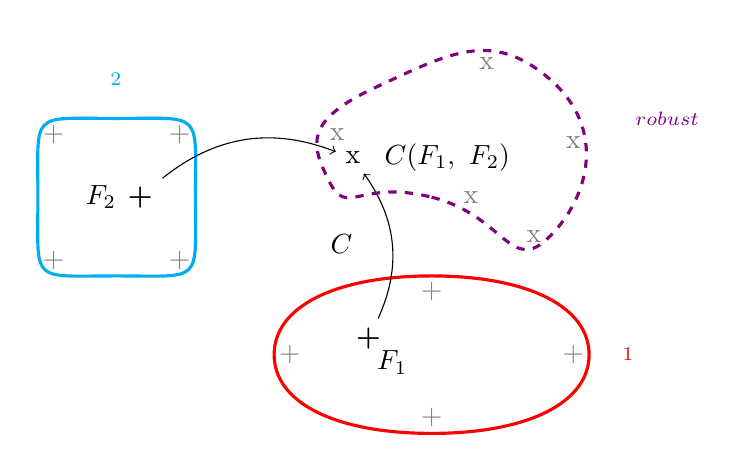
\begin{tikzpicture}[scale=1]
        \draw [red, line width=0.4mm] plot [smooth cycle, tension=1.1] coordinates {(5,1) (7,2) (5,3) (3,2)};
        \draw [cyan, line width=0.4mm] plot [smooth cycle, tension=2] coordinates {(0,4) (1,3) (2,4) (1,5)};
        
        \draw (7.5, 2) node (Belx) {\color{red}$\M_1$};
        \draw (1, 5.5) node (Bely) {\color{cyan}$\M_2$};
        
        \draw (4.2, 2.2) node (a) {\textbf{+}};
        \draw (4.5, 1.9) node (A) {$F_1$};
        \draw [gray] (5, 1.2) node (+) {+};
        \draw [gray] (6.8, 2) node (+) {+};
        \draw [gray] (5, 2.8) node (+) {+};
        \draw [gray] (3.2, 2) node (+) {+};
        
        
        \draw (1.3, 4) node (b) {\textbf{+}};
        \draw (0.8, 4) node (B) {$F_2$};
        \draw [gray] (0.2, 3.2) node (+) {+};
        \draw [gray] (0.2, 4.8) node (+) {+};
        \draw [gray] (1.8, 3.2) node (+) {+};
        \draw [gray] (1.8, 4.8) node (+) {+};
        
        \draw (4, 4.5) node (c) {x};
        \draw (5.2, 4.5) node (C) {$C(F_1,~F_2)$};
        \draw[->] (a) to [bend right] node[midway, left, inner sep=0.5cm] {$C$}(c);
        \draw[->] (b) to [bend left] (c);
        
        \draw [gray] (3.8, 4.8) node (c) {x};
        \draw [gray] (6.8, 4.7) node (c) {x};
        \draw [gray] (5.7, 5.7) node (c) {x};
        \draw [gray] (6.3, 3.5) node (c) {x};
        \draw [gray] (5.5, 4) node (c) {x};
        
        \draw [violet, dashed, line width=0.4mm] plot [smooth cycle,tension=1.2] coordinates {(3.7, 4.2) (5, 4) (6.5, 3.5) (6.5, 5.5) (4.3, 5.4)};
        
        \draw (8, 5) node (robust) {\color{violet}{$\M_{robust}$}};
    \end{tikzpicture}
    \caption{Schematic representation of $\M_{robust}$}\label{fig:schema_m_robust}
\end{figure}

\subsection{Copula Applied to Cumulative Mass Functions}\label{sec:joint_mass}
In this section, we will present another way of creating a joint credal set from multiple marginal ones. Consider the same copula $C$ as before and the same marginal credal sets $\M_i$. Each credal set $\M_i$ is fully determined by a mass distribution function $m_i$, which is strictly positive over its $N_i$ focal sets $a^i_1 \enum a^i_{N_i}$. As described in \cite{ferson_dependence_2004}, it is possible to use the cumulative mass distribution functions as marginals of the copula to create a joint mass distribution function, granted that there is a complete ordering defined on the focal sets. Links between copulas and belief functions have been investigated in the continuous case in \cite{schmelzer_joint_2015, schmelzer_multivariate_2019}, the special case of necessity functions in \cite{schmelzer_sklars_2015} and of p-boxes in \cite{schmelzer_random_2023}.

Let us assume, without loss of generality, that the marginal focal sets are numbered according to the ordering $\preceq_i$: $a^i_1\preceq_ia^i_2\preceq_i\ldots\preceq_i a^i_{N_i}$. The idea behind this method is to replace the precise marginal \acrshort{cdf}s by cumulative masses, to keep the philosophy behind \hyperref[theorem:sklar]{Sklar's Theorem}. We thus first define the joint mass $m_C$ on the product space of focal sets as follows:

\begin{definition}[Joint Mass]\label{def:joint_mass}
    Let $m_1 \enum m_n$ be mass distribution functions over their respective power sets of $\X_1 \enum \X_n$. Assume that focal sets in each $\X_i$ are ordered and that $a_{k_i}^i$ is the $k_i$-th focal set of $m_i$ according to the chosen order. We define $m_C$ as the H-volume of copula $C$ computed over the cumulative marginal masses:
    \begin{eqnarray}\label{eq:joint_mass}
        m_C(a^1_{k_1}\tdt a^n_{k_n}) = H_{\sum_{k=0}^{k_1-1}m_1(a^1_k) \enum \sum_{k=0}^{k_n-1}m_n(a^n_k)}^{\sum_{k=0}^{k_1}m_1(a^1_k) \enum \sum_{k=0}^{k_n}m_n(a^n_k)}
    \end{eqnarray}
    with the convention that $\forall i,\, a^i_0=\emptyset$. It is not \textit{strictly} a focal set but allows dealing with the case $k_i=1$ as $m_i(a^i_0)=0$. For sets that are not of the form $a^1_{k_1}\tdt a^n_{k_n}$, the mass $m_C$ is null.
\end{definition}

\begin{proposition}
    The function $m_C$ defined in \Cref{eq:joint_mass} is a correctly defined mass distribution function over $\X$. 
\end{proposition}
\begin{proof}
    To be a mass distribution function over $\X$, $m_C$ must verify the 3 properties of \Cref{def:mass_distribution_function}.
    
    By construction, it holds that $m_C(\emptyset)=0$, and the properties of the H-volume impose that $m_C\in[0,1]$.
    
    There are multiple ways of proving that $\sum_{A\subseteq\X}m_C(A)=1$. A direct proof can be done in the case $n=2$, but the notations become quite heavy for any $n>2$. Instead, let us use the interpretation of a copula as a multivariate \acrshort{cdf}. This method will also be used in future proofs.
    
    For all \(i\in\opi 0,\, n\cli\) let $F_i$ be a \acrshort{cdf} over $[0,\, N_i]$, with $F_i(j)=\sum_{k=0}^j m_i(a_k^i)$. By \hyperref[theorem:sklar]{Sklar's Theorem}, $F=C(F_1 \enum  F_n)$ is a multivariate \acrshort{cdf} over $[0,\, N_1]\tdt[0,\, N_n]$, and $P$ its \acrshort{pdf}. Thus, it holds that $P([0,\, N_1]\tdt[0,\, N_n])=F(N_1,\ldots,N_n)=1$ and:
    \begin{eqnarray*}
        P([0, N_1]\tdt[0, N_n]) &=& P([0, ~\ldots, ~0])+\\
        &&P\left(\bigsqcup_{k_1=0}^{N_1-1}\ldots\bigsqcup_{k_n=0}^{N_n-1}\left(]k_1, k_1+1]\tdt]k_n, k_n+1]\right)\right)\\
        &=& 0 + \sum_{k_1=0}^{N_1-1}\ldots\sum_{k_n=0}^{N_n-1} P(]k_1, k_1+1]\tdt]k_n, k_n+1])\\
        && \text{(\acrshort{cdf} of a union of disjoint elements, as in \Cref{fig:Demo_CDF})}\\
        &=& \sum_{k_1=0}^{N_1-1}\ldots\sum_{k_n=0}^{N_n-1} H_{F_1(k_1) \enum F_n(k_n)}^{F_1(k_1+1) \enum F_n(k_n+1)}\\
        &=& \sum_{k_1=1}^{N_1}\ldots\sum_{k_n=1}^{N_n} H_{\sum_{k=0}^{k_1-1}m_1(a^1_k) \enum \sum_{k=0}^{k_n}m_n(a^n_k)}^{\sum_{k=0}^{k_1}m_1(a^1_k) \enum \sum_{k=0}^{k_n}m_n(a^n_k)}\\
        &=& \sum_{(a^1_{k_1}\tdt a^n_{k_n})\subseteq\X}m_C(a^1_{k_1}\tdt a^n_{k_n})
    \end{eqnarray*}
Therefore it holds that:
\begin{eqnarray}
    \sum_{A\subseteq\X}m_C(A)=\sum_{(a^1_{k_1}\tdt a^n_{k_n})\subseteq\X}m_C(a^1_{k_1}\tdt a^n_{k_n})=1
\end{eqnarray}
which proves that $m_C$ is a mass distribution function.

{\centering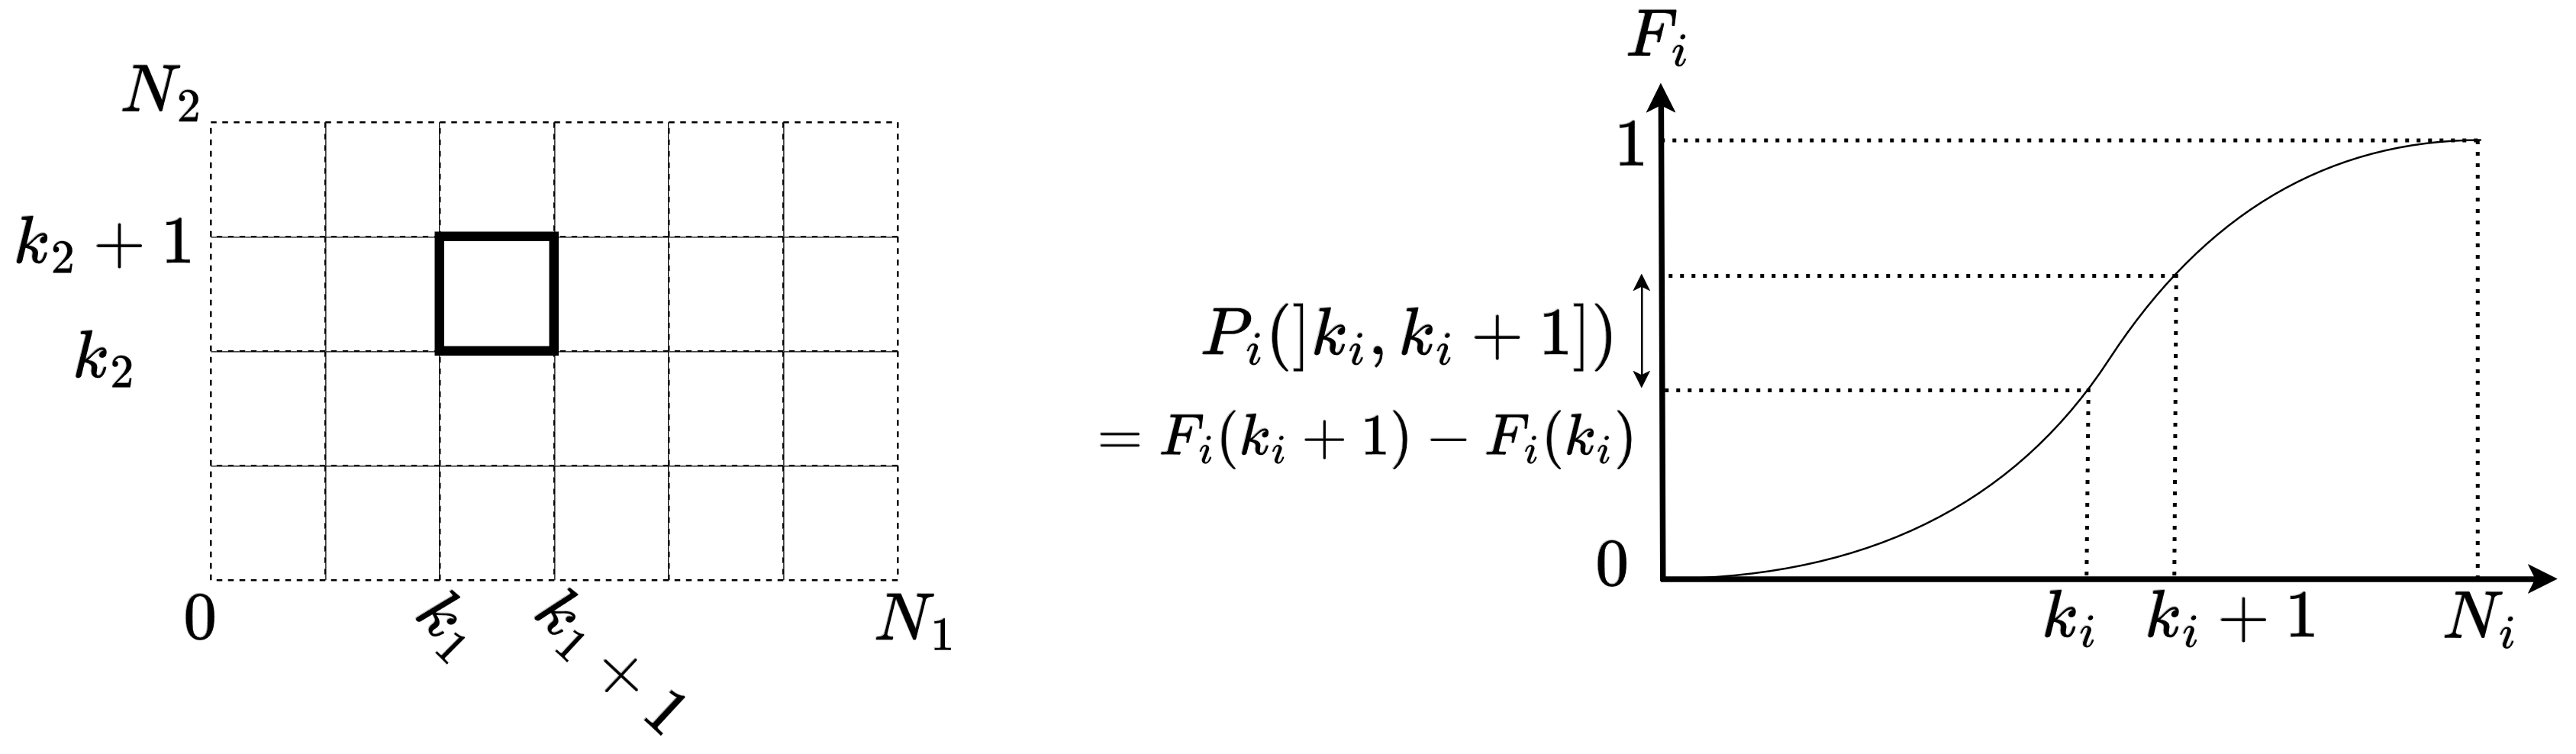
\includegraphics[width=\linewidth]{Images/Chap_3/Demo_CDF.png}\captionof{figure}{Splitting a \acrshort{cdf} into a sum of disjoint events in dimension 1}\label{fig:Demo_CDF}}\par
\end{proof}

Having defined a mass distribution function on the product space $\X$, we thus define the joint credal set $\M_{mass}$ and its belief function $\Bel_C$ as:
\begin{definition}[Joint Belief Function and its Credal Set]\label{def:cumulative_masses_credal_set}
    Let $m_C$ be the mass distribution function from \Cref{def:joint_mass}. We note $\Bel_C$ its joint belief function over the power set of $\X=\X_1\tdt \X_n$, \ie:
    \begin{align}
        \forall A\subseteq\X, \Bel_C(A)=\sum_{a\subseteq A}m_C(a)\label{eq:joint_belief}
    \end{align}
    Because $\Bel_C$ is a belief function, it defines a credal set $\M_{mass}$:
    \begin{eqnarray}
        \M_{mass}(C,\M_i) = \{~P:2^\X\rightarrow [0,1] ~|~ \forall A\subseteq\X, P(A)\geqslant \Bel_C(A)~\}\label{eq:credal_set_mass}
    \end{eqnarray}
    We only specify the lower bound $\Bel_C$ in the expression of the credal set as 
    \begin{align*}
        \Bel_C(A^c)&\leqslant P(A^c)\\
        \Leftrightarrow 1-\Pl(A) &\leqslant 1-P(A)\\
        \Pl(A) &\geqslant P(A)
    \end{align*}
\end{definition}

\Cref{fig:schema_credal_mass} presents a schematic of $\Bel_C$ similarly to what was presented with $\M_{robust}$ in \Cref{fig:schema_m_robust}: $\Bel_C$ is computed from $\Bel_1$ and $\Bel_2$. The gray ``+'' and ``X'' signs have the same position as in \Cref{fig:schema_m_robust}, which shows that $\M_{robust}$ and $\M_{mass}$ are not the same, as the copula is applied to the cumulative masses instead of being applied point-wise to every \acrshort{cdf} from marginal sets.
\begin{figure}
    \centering
    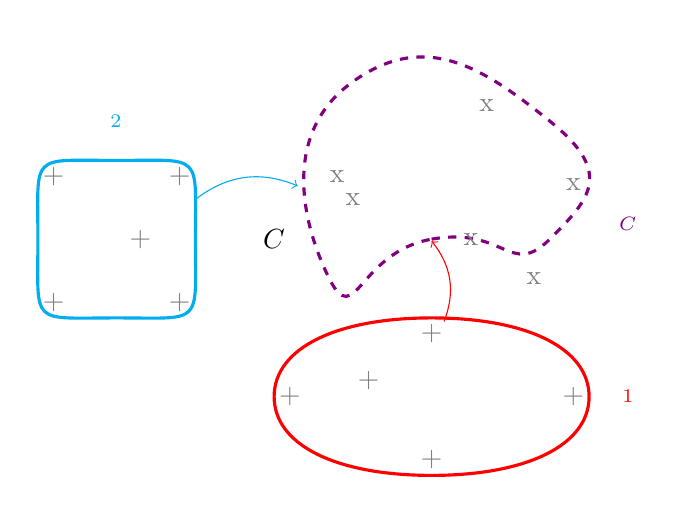
\begin{tikzpicture}[scale=1]
        \draw (7.5, 2) node (Belx) {\color{red}$\Bel_1$};
        \draw (1, 5.5) node (Bely) {\color{cyan}$\Bel_2$};
        
        \draw (5.1, 2.83) node (a) {};
        \draw (5, 4.1) node (b) {};
        \draw (1.88, 4.4) node (c) {};
        \draw (3.3, 4.8) node (d) {};
        
        \draw[->, red] (a) to [bend right] node[midway, left, inner sep=0.5cm] {} (b.south);
        \draw[->, cyan] (c) to [bend left] node[midway, left, inner sep=0.5cm] {} (d.south);
        \draw (3, 4) node (e) {$C$};
        
        \draw [red, line width=0.4mm] plot [smooth cycle, tension=1.1] coordinates {(5,1) (7,2) (5,3) (3,2)};
        \draw [cyan, line width=0.4mm] plot [smooth cycle, tension=2] coordinates {(0,4) (1,3) (2,4) (1,5)};
        \draw [violet, dashed, line width=0.4mm] plot [smooth cycle,tension=1.2] coordinates {(3.7, 3.5) (5, 4) (6.5, 4) (6.5, 5.5) (4, 6) };
        
        \draw (7.5, 4.2) node (mass) {\color{violet}$\Bel_C$};
        
        \draw [gray] (4.2, 2.2) node (+) {+};
        \draw [gray] (5, 1.2) node (+) {+};
        \draw [gray] (6.8, 2) node (+) {+};
        \draw [gray] (5, 2.8) node (+) {+};
        \draw [gray] (3.2, 2) node (+) {+};
        
        \draw [gray] (1.3, 4) node (+) {+};
        \draw [gray] (0.2, 3.2) node (+) {+};
        \draw [gray] (0.2, 4.8) node (+) {+};
        \draw [gray] (1.8, 3.2) node (+) {+};
        \draw [gray] (1.8, 4.8) node (+) {+};
        
        \draw [gray] (4, 4.5) node (x) {x};
        \draw [gray] (3.8, 4.8) node (x) {x};
        \draw [gray] (6.8, 4.7) node (x) {x};
        \draw [gray] (5.7, 5.7) node (x) {x};
        \draw [gray] (6.3, 3.5) node (x) {x};
        \draw [gray] (5.5, 4) node (x) {x};
    \end{tikzpicture}
    \caption{Schematic representation of $\M_{mass}$} \label{fig:schema_credal_mass}
\end{figure}

With this way of defining the multivariate mass, the choice of arbitrary orderings $\preceq_i$ can have a significant impact on the value of the multivariate mass function, as we will see in example \Cref{ex:joint_mass}. Those orderings will specifically be ``natural'' orderings in \Cref{sec:necessity_functions,subsec:pboxes,subsec:multiple_models}, in the sense that there exists an intuitive total ordering (inspired by the ordering of reals). When no natural ordering exists, the arbitrary choice of the ordering can greatly impact the output mass or belief functions, as illustrated by the following example.
\begin{example}\label{ex:joint_mass}
    Let us consider the same setting as \Cref{ex:robust_credal_set} with two coins, and their mass defined this time as:\newline\medskip
    \begin{minipage}{0.5\linewidth}
    	\begin{align*}
    		&m_1(heads)=0.4 \\
    		&m_1(\X_1)=0.6
    	\end{align*}
    \end{minipage}
    \begin{minipage}{0.5\linewidth}
    	\begin{align*}
    		&m_2(tails)=0.7\\
    		&m_2(\X_2)=0.3
    	\end{align*}
    \end{minipage}\bigskip\newline
   We consider the minimum copula $C(u,v)=\min(u,v)$ 
    If there is no natural ordering on the focal sets of $m_1$, we have to choose an arbitrary one:\par
    $\bullet$ If "$\{heads\}\preceq_1 \X_1$" and "$\{tails\}\preceq_2\X_2$" are the arbitrary orderings, then
    \begin{eqnarray*}
        \Bel_C(heads,tails) &=& m_C(heads,tails)\\
        &=&C\left(m_1(heads),~m_2(tails)\right)\\
        &=& \min(0.4,0.7)\\
        &=&0.4
    \end{eqnarray*}\par
    $\bullet$ If "$\X_1\preceq_1 \{heads\}$" is the arbitrary order, then
    \begin{eqnarray*}
        \Bel_C(heads,tails) &=& m_C(heads,tails)\\
        &=&C\left(1,~m_2(tails)\right) - C\left(m_1(\X_1),~m_2(tails)\right)\\
        &=& m_2(tails) -\min(0.6,~0.7)\\
        &=& 0.1
    \end{eqnarray*}
    This illustrates that different orderings lead to different masses and thus to different credal sets.
\end{example}

\begin{remark}
    One reason why $\M_{robust}$ is usually different from $\M_{mass}$ is mainly because the ordering on focal sets can greatly differ from the ordering on reals. Consider for instance the minimum copula already presented in \Cref{ex:copulas}:
    \begin{itemize}
        \item In the precise setting, the minimum copula associates the highest probabilities to events with similar values (high-high or low-low), and the lowest probabilities to events with opposite values (low-high).
        \item In the imprecise setting, the concept of high or low values for focal sets does not usually exist. We thus replace it by an ordering $\preceq$ on focal sets, determining which set is considered ``low'' and which is ``high'' (regardless of the real values actually contained in the set). The minimum copula then associates the highest mass to joint focal sets with similar ``values'' in the sense of the ordering $\preceq$, and the lowest mass to sets with opposite values in the sense of the ordering $\preceq$. For instance, in the bivariate case, with marginal focal sets $a_1^1\preceq_1 a_2^1$ and $a^2_1\preceq_2 a^2_2$, using the minimum copula will assign high masses to $a^1_1\times a^2_1$ and $a^1_2\times a^2_2$ and low masses to $a^1_1\times a^2_2$ and $a^1_2\times a^2_1$.
    \end{itemize}
    Assigning a high mass to sets containing both low and high values at the same time is something that would not occur in the precise case, but is possible in the imprecise case. This explains a source of the difference between credal sets $\M_{mass}$ and $\M_{robust}$. 
\end{remark}

We saw that $\M_{robust}$ and $\M_{mass}$ can be different credal sets. However, because $\M_{robust}$ is difficult to compute, it would be interesting to still use $\M_{mass}$ to approximate it, \ie to verify that $\M_{robust}\subseteq\M_{mass}$ (outer approximation) or $\M_{mass}\subseteq\M_{robust}$ (inner approximation). In \Cref{ex:mass_values}, we show that there is in general no reason for such a relation to exist. Furthermore, if we found an ordering allowing this relationship, then this ordering is copula dependent, as changing the copula might break the inclusion. 
\begin{example}\label{ex:mass_values}
    Consider the following setting:
    \begin{itemize}
        \item We consider two spaces $\X_1=\X_2=\{1,~2,~3\}$
        \item We consider two (identical) mass distribution functions $m_1$, $m_2$, each respectively possessing two focal sets $\{2\}$ and $\{1,3\}$.
        \item $m_1(\{2\}) = m_1(\{1,~3\}) = m_2(\{2\})= m_2(\{1,~3\}) = 0.5$
        \item We want to join the credal sets induced by the mass functions using the minimum copula.
    \end{itemize}
    We will compute the bounds of $\M_{mass}$ and $\M_{robust}$ to compare them. The marginals masses being identical and the copula being symmetrical, many results can be obtained by symmetry.
    
    Let us first compute the bounds of $\M_{robust}$. Marginal masses $m_1$  and $m_2$ imposes that each marginal probability $P_1\in\M_1$ will verify:
    \begin{align*}
        \Bel_1(\{2\}) \leqslant &P_1(\{2\}) \leqslant \Pl_1(\{2\})\\
        0.5 = \sum_{a\subseteq\{2\}}m_1(a) \leqslant &P_1(\{2\}) \leqslant \sum_{a\cap\{2\}\neq\emptyset}m_1(a) = 0.5
    \end{align*}
    The same result holds for $\{1,~3\}$. We therefore have:
    \begin{align*}
        &P_1(2)=0.5\\
        &P_1(1)+P_1(3)=0.5\\
        &0\leqslant P_1(1)\leqslant 0.5\\
        &0\leqslant P_1(3)\leqslant 0.5
    \end{align*}
    And we can compute the same for $m_2$. Looking at those equations, we can deduce that every $P\in\M_{robust}$ with marginals $P_1,P_2$ verifies for events  $\{1\}\times\{1\}$ and $\{1,2\}\times\{1,2\}$:
    \begin{align*}
    	&P(\{1\},~ \{1\}) = \min(P_1(1), P_2(1))\\
        \implies 0 = \min(0, 0)  \leqslant ~&P(\{1\},~ \{1\}) ~\leqslant \min(0.5, 0.5) = 0.5\\
        &P(\{1, ~2\},~ \{1, ~2\}) = \min(P_1(\{1, ~2\}), P_2(\{1, ~2\}))\\
        \implies 0.5 = \min(0+0.5, 0.5+0) \leqslant ~&P(\{1, ~2\},~ \{1, ~2\}) ~\leqslant min(0.5+0.5, 0.5+0.5)=1
    \end{align*}
    
    Let us now compute the bounds of $\M_{mass}$. Choosing an ordering between $\{1, ~3\}$ and $\{2\}$ is not intuitive. Assume that there is a reason which encourages us to choose different orderings for the focal sets of $m_1$ and for those of $m_2$, so that $\{1,~3\} \preceq_1 \{2\}$ and $\{2\} \preceq_2 \{1,~3\}$. In this case, using \Cref{eq:joint_mass} it holds that:
    \begin{align*}
        m_C(\{1, ~3\}, \{2\}) =& ~\min(0.5, ~0.5)\\
        =& ~0.5\\
        m_C(\{2\}, \{1, ~3\}) =& ~\min(1, ~1) - \min(0.5, ~1)\\
        & - \min(1, ~0.5) + \min(0.5, ~0.5)\\
        =& ~0.5\\
        m_C(\{2\}, \{2\}) =& ~0\\
        m_C(\{1, ~3\}, \{1, ~3\}) =& ~0
    \end{align*}
    Thus every probability $P\in\M_{mass}$ will verify:
    \begin{align*}
    	\Bel_C(\{1\},~ \{1\}) \leqslant ~&P(\{1\},~ \{1\})  ~\leqslant \Pl(\{1\},~ \{1\}) \\
    	\Leftrightarrow\sum_{a\subseteq(\{1\}\times \{1\})}m_C(a)\leqslant ~&P(\{1\},~ \{1\})  ~\leqslant\sum_{a\cap(\{1\}\times \{1\})\neq\emptyset}m_C(a)\\
        \Leftrightarrow 0 \leqslant ~&P(\{1\},~ \{1\}) ~ \leqslant 0
    \end{align*}
    and
     \begin{align*}
        \Bel_C(\{1, ~2\},~ \{1, ~2\}) \leqslant ~&P(\{1, ~2\},~ \{1, ~2\})  ~\leqslant \Pl(\{1, ~2\},~ \{1, ~2\}) \\
        \Leftrightarrow\sum_{a\subseteq(\{1, ~2\},~ \{1, ~2\})}m_C(a)\leqslant ~&P(\{1, ~2\},~ \{1, ~2\})  ~\leqslant\sum_{a\cap(\{1, ~2\},~ \{1, ~2\})\neq\emptyset}m_C(a)\\
        \Leftrightarrow 0 \leqslant ~&P(\{1, ~2\},~ \{1, ~2\})~ \leqslant 1
    \end{align*}
 
    Looking at the bounds of $\M_{mass}$ and $\M_{robust}$ on cumulative event $\{1\}\times\{1\}$, we can see that $\overline{P}_{robust}(\{1\}, \{1\}) > \Pl(\{1\}, \{1\}))$ and thus $\M_{robust}\not\subseteq \M_{mass}$.
    Looking at the bounds on $\{1,2\}\times\{1,2\}$, we can see that $\low_{robust}(\{1, ~2\},~ \{1, ~2\}) > \Bel_C(\{1, ~2\},~ \{1, ~2\})$ and thus $\M_{mass}\not\subseteq \M_{robust}$.
    
    \begin{remark}
        The bounds of $\M_{mass}$ depend both on the ordering and the copula used. Therefore, if an ordering exists such that $\M_{robust}\subseteq\M_{mass}$ or $\M_{mass}\subseteq\M_{robust}$, then this ordering is not guaranteed to keep the inclusion relationship using a different copula.
    \end{remark}
\end{example}

We considered until now that an ordering has to be chosen arbitrarily. However, special cases of belief functions exhibit a natural ordering on their focal sets, for instance p-boxes and possibilities. Those special cases will be explored in \Cref{sec:inclusions_between_methods}.

\subsection{Copulas Applied to Belief Functions}\label{sec:aggregation_method}
Another way of joining credal sets with a copula is by directly applying the copula to their lower envelope $\low_i$ for every event:
\begin{definition}[Aggregated Credal Set]\label{def:aggregation_credal_set}
    Given a copula $C$ and $n$ marginal credal sets whose lower probabilities are $\low_1 \enum \low_n$, we define the credal set $\M_{agg}$ over the power set of $\X=\X_1\tdt X_n$ as:
    \begin{eqnarray}
        \M_{agg} = CH(\{P ~|~\forall A_i\subseteq\X_i, P(A_1 \enum  A_n)\geqslant C(\low_1(A_1) \enum \low_n(A_n))\})\nonumber\\
        \,\label{eq:copula_on_lower_proba}
    \end{eqnarray}
    where $CH$ is the convex hull from \Cref{def:convex_hull}.
\end{definition}

Contrary to $\M_{mass}$ or $\M_{robust}$, constraints on this set only occur on Cartesian products in $\X$. We thus take the convex hull for extending its definition to every event in $2^\X$. We denote this credal set as $\M_{agg}$ because it uses the copula solely as an aggregation operator, without conserving the meaning associated with copulas by \hyperref[theorem:sklar]{Sklar's Theorem}. In this regard, $\M_{agg}$ has less meaning than $\M_{robust}$ or $\M_{mass}$, but presents the advantage of being easier to compute on cylindrical sets. \Cref{fig:meaning_computation} sums up the performances of the different methods in terms of computation cost and meaningfulness.

\begin{figure}[!hb]
    \centering
    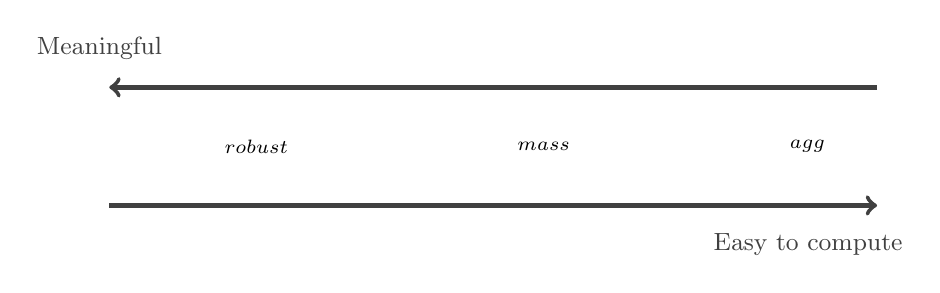
\begin{tikzpicture}[scale=1]
        \draw (0, 0) node (a) {};
        \draw (10, 0) node (b) {};
        \draw (0, 1.5) node (c) {};
        \draw (10, 1.5) node (d) {};
        
        \draw[->, ultra thick, darkgray] (a) to node[midway, left, inner sep=0.5cm] {} (b);
        \draw[->, ultra thick, darkgray] (d) to node[midway, left, inner sep=0.5cm] {} (c);
        
        \draw [darkgray] (9, -0.5) node (z) {\small Easy to compute};
        \draw [darkgray] (0, 2) node (z) {\small Meaningful};
        
        \draw (9, 0.75) node (z) {$\M_{agg}$};
        \draw (5.65, 0.75) node (z) {$\M_{mass}$};
        \draw (2, 0.75) node (z) {$\M_{robust}$};
    \end{tikzpicture}
    \caption{Comparing different methods of joining credal sets with a copula.}
    \label{fig:meaning_computation}
\end{figure}

In general, applying the copula directly to the lower probabilities as in \eqref{eq:copula_on_lower_proba} does not produce a coherent lower probability inducing a non-empty credal set (see \Cref{def:coherence_sure_loss}). For instance, let us consider $\X_1 = \X_2 = \{1, 2\}$, two lower previsions $\low_1$ and $\low_2$ such that $\low_1(\{1\}) = \low_1(\{2\}) = \low_2(\{1\}) = \low_2(\{2\}) = 0.5$. Joining those two lower probabilities using the minimum copula $C(u,v)=\min(u,v)$ gives a mapping $\low$ which induces an empty credal set, as presented in \Cref{tab:non_coherent_lower}. Indeed, no probabilities can satisfy all these constraints at once. 

\begin{table}[!ht]
    \centering
    \begin{tabular}{|c||c|c|}
        \hline
        \hspace{0.2cm} $\low$ \hspace{0.2cm} & \hspace{0.2cm} $\{1\}$ \hspace{0.2cm} & \hspace{0.2cm} $\{2\}$ \hspace{0.2cm} \\\hline\hline
        $\{1\}$ & $0.5$ & $0.5$ \\\hline
        $\{2\}$ & $0.5$ & $0.5$\\
        \hline
        \end{tabular}
        \caption{$\low = \min(\low_1, \low_2)$}
        \label{tab:non_coherent_lower}
\end{table}

\begin{proposition}
    In the special case of the product copula $C_\Pi$, the credal set $\M_{agg}$ induced by \eqref{eq:copula_on_lower_proba} is not empty. It follows that for all copulas $C$ dominated by the product copula (\ie $C_\Pi\geqslant C$), and for every non-empty marginal credal set $\M_i$, $\M_{agg}(C, \M_i)$ is also non-empty credal set.
\end{proposition}

\begin{proof}
    For $i\in\{1 \enum n\}$, let $\low_i$ be a lower probability avoiding sure loss, \ie whose credal set $\M_i$ contains at least one probability distribution $P_i$. Let us define a multivariate probability $P$ on every $(A_1\tdt A_n)\subseteq\X$ as:
    \begin{eqnarray*}
        P(A_1\tdt A_n) = P_1(A_1)\tdt P_n(A_n)
    \end{eqnarray*}
    Defining $P$ on $(A_1\tdt A_n)\subseteq\X$ is sufficient as those sets contain every atom of $\X$.
    Because $\forall i, P_i\in\M_i,~P_i\geqslant \low_i$, then:
    \begin{eqnarray*}
        P(A_1\tdt A_n) \geqslant \low_1(A_1)\tdt \low_n(A_n) &=& C_\Pi(\low_1(A_1) \enum \low_n(A_n))\\
        &=& \low_{C_\Pi}(A_1\tdt A_n)
    \end{eqnarray*}
which means $P\in\M_{agg}(C_\Pi, \M_i)$. Therefore, $\M_{agg}(C_\Pi, \M_i)\neq\emptyset$ if every $\M_i\neq\emptyset$.

Let $C$ be a copula dominated by $C_\Pi$ (\ie $C_\Pi\geqslant C$), and $\low_C$ the lower probability associated with $\M_{agg}(C, \M_i)$. Then it holds that for all $(A_1\tdt A_n)\subseteq\X$:
\begin{eqnarray*}
\low_{C_\Pi}(A_1\tdt A_n)&=&C_\Pi(\low_1(A_1) \enum \low_n(A_n)) \\
    &\geqslant& C(\low_1(A_1) \enum  \low_n(A_n)) = \low_C(A_1\tdt A_n)
\end{eqnarray*}
which implies that $\M_{agg}(C_\Pi, \M_i)\subseteq \M_{agg}(C, \M_i)$. Therefore, if every $\M_i$ is a non-empty credal set, then $ \M_{agg}(C, \M_i)$ is also non-empty.
\end{proof}

\begin{proposition}
    Conversely, no lower probability $\low_C$ obtained using \eqref{eq:copula_on_lower_proba} with a copula $C$ strictly superior to the product copula is guaranteed to induce a non-empty credal set $\M_{agg}$. It all depends on the marginal credal sets $\low_i$.
\end{proposition}

\begin{proof}
    Let $C$ be a copula strictly superior to the product. Then there exists $(u_1 \enum u_n)\in[0,1]^2$ such that:
    \begin{eqnarray*}
        C(u_1 \enum  u_n)~>~\prod_{i=1}^n u_i
    \end{eqnarray*}
    Let $\M_i$ be marginals credal sets such that $\low_i$ are \textit{precise} probabilities, and that:
    \begin{eqnarray*}
        \forall i,~\exists A_i\in\X_i,~\low_i(A_i)=u_i
    \end{eqnarray*}
    We will prove the proposition by contradiction. Assume that $\M_{agg}(C, \M_i)$ avoids sure loss, \ie there is a probability $P$ such that $P\geqslant\low_C$.  Let $S$ be a collection of disjoint cylindrical sets of $\X$ (defined in \Cref{eq:cylindrical_sets}) covering the complementary event $(A_1\tdt A_n)^c$ of $(A_1\tdt A_n)$. $S$ is defined so that $(A_1\tdt A_n)^c=\bigsqcup_{s\in S}s$.
    Then,
    \begin{eqnarray*}
        P(\X) &=& P\left(\left(A_1\tdt A_n\right)\bigsqcup\left(A_1\tdt A_n\right)^c\right)\\
        &=& P\left(A_1\tdt A_n\right)+P\left((A_1\tdt A_n)^c\right)\\
        &=& P\left(A_1\tdt A_n\right)+\sum_{(s_1\tdt s_n)\in S}P(s_1\tdt s_n)\\
        &\geqslant& \low_C\left(A_1\tdt A_n\right)+\sum_{(s_1\tdt s_n)\in S}\low_C(s_1\tdt s_n)\\
        &>& \low_{C_\Pi}\left(A_1\tdt A_n\right)+\sum_{(s_1\tdt s_n)\in S}\low_{C_\Pi}(s_1\tdt s_n)
    \end{eqnarray*}
    Because we chose $\low_i$ so that they are precise probabilities, their product is also a precise probability. Using the fact that summing probabilities of disjoint events is equal to the probability of their union:
    \begin{eqnarray*}
        \low_{C_\Pi}\left(A_1\tdt A_n\right)+\sum_{(s_1\tdt s_n)\in S}\low_{C_\Pi}(s_1\tdt s_n) &=& \low_{C_\Pi}\left(A_1\tdt A_n\right)+\\
        &&\low_{C_\Pi}\left((A_1\tdt A_n)^c\right)\\
        &=& 1
    \end{eqnarray*}
    This means that $P(\X)>1$ which is impossible. Thus, $\M_{agg}(C, \M_i)=\emptyset$ and $\M_{agg}(C, \M_i)$ does not avoid sure loss.
\end{proof}

We have now presented three methods for joining imprecise models using a copula. The following sections will explore special cases where some interesting relationships between those copulas exist. 

\section{Inclusions Between Joint Credal Sets}\label{sec:inclusions_between_methods}
\Cref{sec:methods_for_joining_credal_sets} presented three methods for joining marginal credal sets using a copula. In general, there is no reason for the three methods to lead to the same multivariate credal sets. However, for some specific cases on the copulas or on the marginal credal sets, it is possible to find inclusion relationships between the methods. This section explores some of these specific cases. Because each method has a different computational complexity, knowing those relationships allows us to use a simpler method to approximate another. For instance, if we know that $\M_{robust}\subseteq\M_{mass}$, then we can determine conservative bounds on $\M_{robust}$ by computing those of $\M_{mass}$, which are simpler to determine. This will specifically be used in \Cref{chap:propagating}.

\subsection{Using the Product Copula}\label{subsection:product_copula}
In this section, we will consider the case of the product copula $C_\Pi$, representing independence between variables. Using this copula in the robust approach defined by \Cref{eq:robust_set} is referred to as the strong product in \cite{kacprzyk_factorisation_2010}. Let us denote $\low_{robust}$ the infimum of $\M_{robust}(C_\Pi, \M_i)$ and $\mathcal{S}$ the set from which $\M_{robust}$ is computed (\Cref{eq:robust_ancestor}).
For cylindrical sets $(A_1 \enum A_n)$ of $\X$, it holds that:
\begin{eqnarray*}
    \low_{robust}(A_1\tdt A_n) &=& \inf\{P(A_1\tdt A_n)~|~P\in\mathcal{S}\}\\
    &=&\inf\{P_1(A_1)\ldots P_n(A_n)~|~P_i\in\M_i\}\\
    &=&\inf\{P_1(A_1)~|~P_1\in\M_1\}\ldots\inf\{P_n(A_n)~|~P_n\in\M_n\}\\
    &=&\low_1(A_1)\ldots\low_n(A_n)
\end{eqnarray*}
We can split the infimum of a product as a product of infima because we consider mappings with positive values. As this is equivalent to applying the copula directly to the marginals, $\M_{robust}$ and $\M_{agg}$ have the same bounds on cylindrical events. On other events, the lower probabilities are defined as the infimum of the credal sets, thus all bounds are the same. $\M_{robust}$ is defined as the convex hull of the set of probabilities whose marginals are in $\M_i$, which is a constraint that $\M_{agg}$ do not have. Therefore, the sets are not necessarily the same, although they share the same bounds. The way $\M_{agg}$, is defined, it is the largest set with those bounds. On the other hand, as $\M_{robust}$ is the convex hull of the set $S$ from \Cref{eq:robust_ancestor} now defined specifically as:
\begin{align*}
    S=\{~F~|&~\forall (x_1\enum x_n)\in\X,~\forall F_i\in\M_i,\\
    &F(x_1\enum x_n)=F_1(x_1)\cdot\ldots\cdot F_n(x_n)~\}
\end{align*}
This means that $\M_{robust}$ is the convex hull of a set of specific probabilities verifying those bounds; it is therefore a smaller set than $\M_{agg}$. It results that:
\begin{eqnarray}
    \M_{robust}(C_\Pi, \M_i)\subseteq\M_{agg}(C_\Pi, \M_i)
\end{eqnarray}
This result can also be found in \cite{couso_survey_2000}.

Let us now consider a property on the mass $m_C$ from \Cref{eq:joint_mass}, which will later allow us to prove an inclusion with $\Bel_C$.
\begin{proposition}
    In the case of the product copula $C_\Pi$, the arbitrary orderings on marginal focal sets have no impact on the value of the joint mass $m_C$ defined in \eqref{eq:joint_mass}. Indeed, if $a^1_{k_1}, ~\ldots, ~a^n_{k_n}$ is a focal set of $m_1, ~\ldots, ~m_n$, then $m_C$ is given by:
    \begin{eqnarray}\label{eq:joint_mass_product}
        m_C(a^1_{k_1}\tdt a^n_{k_n}) = m_1(a^1_{k_1})\ldots m_n(a^n_{k_n})
    \end{eqnarray}
\end{proposition}

\begin{proof}
    For simplicity and coherence with the notations of \Cref{eq:hvolume}, we will note for all $i\in[0,n]$, $u_{k_i}=\sum_{l=0}^{k_i-1}m_i(a_l^i)$, $v_{k_i}=\sum_{l=0}^{k_i-1}m_i(a_l^i)$. $\prod_{i=1}^n\{u_{k_i}, v_{k_i}\}$ will refer to the Cartesian product $\{u_{k_1}, v_{k_1}\}\times\{u_{k_2}, v_{k_2}\}\tdt\{u_{k_n}, v_{k_n}\}$ and we will note $C_\Pi$ and $H$ as the product copula and its H-volume regardless of their number of marginals. Those notations established, it holds that:
    \begin{eqnarray*}
        m_C(a^1_{k_1}\tdt a^{n}_{k_{n}}) &=& H_{u_{k_1} \enum u_{k_n}}^{v_{k_1} \enum v_{k_n}}\\
        &=&\sum_{\substack{(w_{k_1} \enum w_{k_n})\in\\\prod_{i=1}^{n}\{u_{k_i}, v_{k_i}\}}}(-1)^{|\{k~|~w_{k_i}=u_{k_i}\}|}C_\Pi(w_{k_1} \enum w_{k_n})\\
        &=&\sum_{\substack{(w_{k_1} \enum w_{k_n})\in\\\prod_{i=1}^{n}\{u_{k_i}, v_{k_i}\}}}(-1)^{|\{k~|~w_{k_i}=u_{k_i}\}|}(w_{k_1} \cdot\ldots\cdot w_{k_n})
    \end{eqnarray*}
    and by explicitly writing the terms for $w_{k_n}=v_{k_n}$ and $w_{k_n}=u_{k_n}$:
    \begin{eqnarray*}
        m_C(a^1_{k_1}\tdt a^{n}_{k_{n}})&=&\sum_{\substack{(w_{k_1} \enum w_{k_{n-1}})\in\\\prod_{i=1}^{n-1}\{u_{k_i}, v_{k_i}\}}}(-1)^{|\{k~|~w_{k_i}=u_{k_i}\}|}(w_{k_1} \cdot\ldots\cdot w_{k_{n-1}}\cdot v_{k_n})\\
        && + \sum_{\substack{(w_{k_1} \enum w_{k_{n-1}})\in\\\prod_{i=1}^{n-1}\{u_{k_i}, v_{k_i}\}}}(-1)^{|\{k~|~w_{k_i}=u_{k_i}\}|+1}(w_{k_1} \cdot\ldots\cdot w_{k_{n-1}}\cdot u_{k_n})\\
        &=& v_{k_n}H_{u_{k_1} \enum u_{k_{n-1}}}^{v_{k_1} \enum v_{k_{n-1}}} - u_{k_n}H_{u_{k_1} \enum u_{k_{n-1}}}^{v_{k_1} \enum v_{k_{n-1}}}\\
        &=& m_{n}(a^{n}_{k_{n}})H_{u_{k_1} \enum u_{k_{n-1}}}^{v_{k_1} \enum v_{k_{n-1}}}
    \end{eqnarray*}
    Doing the same procedure for every variable leads to:
    \begin{eqnarray*}
        m_C(a^1_{k_1}\tdt a^n_{k_n}) = m_1(a^1_{k_1})\ldots m_n(a^n_{k_n})
    \end{eqnarray*}
    which concludes the proof.
\end{proof}

The mass $m_C$ corresponds to the notion of random set independence presented in \cite{dempster_upper_1967, couso_survey_2000}. Let $\Bel_C$ be the belief function associated with $m_C$, and $\forall i\in[1,n], \Bel_i$ the mass function associated with $m_i$. Then for cylindrical sets $(A_1 \enum A_n)$ of $\X$, it holds that:
\begin{eqnarray}
    \Bel_C(A_1\tdt A_n) &=& \sum_{(a^1\tdt a^n)\subseteq (A_1 \enum A_n)}m_C(a^1\tdt a^n)\nonumber\\
    &=& \sum_{(a^1\tdt a^n)\subseteq (A_1 \enum A_n)}m_1(a_1)\cdot\ldots\cdot m_n(a^n)\nonumber\\
    &=& (\sum_{a^1\subseteq A_1}m_1(a^1))\cdot\ldots\cdot(\sum_{a^n\subseteq A_n}m_n(a^n))\nonumber\\
    &=& \Bel_1(A_1)\ldots \Bel_n(A_n)
\end{eqnarray}

This means that in the case of the product copula $C_\Pi$ with marginals being belief functions, $\M_{robust},~\M_{mass}$ and $\M_{agg}$ all coincide on cylindrical sets. Because $\M_{agg}$ has no specific constraints on other sets, it is the largest credal set with these bounds. Because $m_{mass}$ is defined on other bounds, $\M_{mass}$ also has constraints on other bounds. It is therefore a smaller set than $\M_{agg}$ and:
\begin{eqnarray*}
    \M_{mass}\subseteq\M_{agg}
\end{eqnarray*}
Finally, it is straightforward to verify that $\M_{mass}$ contains every probability from the set $S$
\begin{align*}
    S=\{~F~|&~\forall (x_1\enum x_n)\in\X,~\forall F_i\in\M_i,\\
    &F(x_1\enum x_n)=F_1(x_1)\cdot\ldots\cdot F_n(x_n)~\}
\end{align*}
of which $\M_{robust}$ is the convex hull. As $\M_{mass}$ is defined by a belief function, it is therefore also convex, therefore:
\begin{eqnarray*}
    \M_{robust}\subseteq\M_{mass}
\end{eqnarray*}
In the case of the product copula, the following inclusion ordering holds:
\begin{align}
    \M_{robust}\subseteq\M_{mass}\subseteq\M_{agg}
\end{align}
Regardless of the marginal belief functions used. This means that computing the bounds of $\M_{agg}$, which is straightforward, allow us to obtain a set containing $\M_{robust}$. We also have seen in this section that on Cartesian products, the multivariate belief function could simply be evaluated without computing its joint mass. The next sections will investigate the relationship between $\M_{robust}$, $\M_{mass}$ and $\M_{agg}$ for other copulas, but with specific types of marginal imprecise models.

\subsection{Using the Natural Ordering of Necessity Functions}\label{sec:necessity_functions}
We will now investigate the specific case where we use any copula $C$ to join multiple marginal necessity functions. This setting will be considered in \Cref{chap:propagating}. We saw in \Cref{sec:possibilities} that focal sets $(a_1\enum a_n)$ of necessity functions are included into one another as follows:
\begin{align*}
    a_1\subset a_2\subset\ldots\subset a_n
\end{align*}
Here, we used a specific ordering for focal sets (the natural order) but any other ordering could have been used. A family of events verifying this inclusion property is called an \textit{increasing} family of events in the following. 

In \cite{schmelzer_joint_2015}, the author showed that in order to describe the relation between a multivariate belief function and its marginals in the bivariate case, it is necessary to consider a family of sub-copulas: one copula for each tuple of increasing family of events. We remind that a sub-copula is a restriction of a copula to a subset of the unit hyper-cube $[0,1]$ as presented in \Cref{sec:copula_def}.

\begin{theorem}[Sklar's Theorem for Belief Functions \cite{schmelzer_joint_2015}]\label{theorem:sklarbelief}
    Let $\Bel :2^{\X_1}\times2^{\X_2}\rightarrow[0,1]$ be a bivariate belief function and let $\Bel_1$ and $\Bel_2$ denote its marginals over $2^{\X_1}$ and $2^{\X_2}$ respectively. Furthermore, let $\mathcal{I}_1$ and $\mathcal{I}_2$ denote increasing families of subsets of $\X_1$ and $\X_2$. Then there exists a unique sub-copula $C^{\mathcal{I}_1,\mathcal{I}_2}$ on  $\Bel_1(\mathcal{I}_1)\times \Bel_2(\mathcal{I}_2)$ such that:
    \begin{eqnarray}
        \Bel (L_1, L_2) = C^{\mathcal{I}_1,\mathcal{I}_2}(\Bel_1(L_1), \Bel_2(L_2))
    \end{eqnarray}
    for all $L_1\in\mathcal{I}_1,L_2\in\mathcal{I}_2$.
\end{theorem}
For the reverse to be true, it is necessary that $\X_1\in\mathcal{I}_1, \X_2\in\mathcal{I}_2$. Example 1 of \cite{schmelzer_joint_2015} illustrate the need of a copula for each increasing family of events.

\begin{remark}
    In \cite{lesniewska-choquet_specialite_2020}, it has been proposed to directly apply the copula to the marginal possibility distributions $\pi_i$, \ie $\pi(x,y)=C(\pi_1(x), \pi_2(y))$. It is however shown that this method does not work in general with copulas; however, the author presents more specific aggregation models (called \textit{t-conorms}) as a solution. This work is very interesting, and is also used on satellite images (although for a different application as ours, \ie for detecting land changes). Although it may seem very similar to our subject, we sadly cannot compare our results to it as the considered settings differ too much. The objective of their thesis can be briefly summed as follows: given a multivariate probability $P$, how to obtain a multivariate possibility distribution $\pi$ consistent with $P$, \ie such that $P\in\M(\pi)$. They also restrict the marginals of $P$ to single probability distributions (and not credal sets), which must be either Gaussian, Cauchy or Student probability distributions. They show that determining such a multivariate possibility is possible for the upper and lower Fréchet–Hoeffding bounds, but can only determine bounds on the possibility for the product copula, for instance. Other copulas are not considered. Linking our work to theirs seemed a big stretch and has thus not be considered. 
\end{remark}

Necessity functions are completely determined by their focal sets, which form an increasing family of events. Thus, by applying \hyperref[theorem:sklarbelief]{Sklar's Theorem for Belief Functions}, it holds that joining two necessity functions with a copula $C$ as in \eqref{eq:copula_on_lower_proba} yields a bivariate belief function (which is not necessarily a necessity function):
\begin{equation}
    \Bel = C(\Nec_1, \Nec_2)\label{eq:sklar_on_necessity}
\end{equation}
where $\Nec_1$ and $\Nec_2$ are the marginal necessity functions. The proof of those results were shown in \cite{schmelzer_joint_2015,schmelzer_sklars_2015}. This way of applying the copula directly on necessities is the same approach as in $\M_{agg}$. In the following, we will consider that the focal sets $a^i$ of a necessity functions $\Nec_i$ are already ranked using the natural ordering $\preceq_i$, which is convenient when manipulating those representations:
\begin{eqnarray}
    \forall (k,j)\in[1, N_i]^2,~k\leqslant j ~\Leftrightarrow ~ a^i_k \preceq_i a^i_j ~\Leftrightarrow ~ a^i_k\subseteq a^i_j
\end{eqnarray}

The method for joining necessity functions from \hyperref[theorem:sklar]{Sklar's Theorem} is similar to the one for creating a multivariate belief function as in \eqref{eq:joint_belief}, as presented in the following proposition.

\begin{proposition}\label{prop:sklar_necessity}
    Joining two marginal necessity functions $\Nec_1, \Nec_2$ with a copula $C$ as in \eqref{eq:sklar_on_necessity} or using the bivariate mass function as in \eqref{eq:joint_mass} with the natural inclusion ordering yields the same bivariate belief function.
\end{proposition}

\begin{proof}
    If we denote by $\Bel_C$ the belief function defined in \eqref{eq:joint_mass} where the ordering is the inclusion ordering $\preceq_i$ for $i\in[1,2]$. For convenience and with respect to the notations of \Cref{eq:hvolume}, we note: $u^i_k=\sum_{j=0}^{k}m_i(a_j^i)$ and consider that $a^i_0=\emptyset$.
    For all focal elements $a_k^1$ of $\Nec_1$ and $a^2_j$ of $\Nec_2$, it holds that:
    \begin{eqnarray*}
        \Bel_C(a^1_k, a^2_j) &=& \sum_{a^1_p\subseteq a_k^1}\sum_{a^2_q\subseteq a_j^2}m_C(a^1_p, a^2_q) = \sum_{p=1}^k\sum_{q=1}^j m_C(a^1_p, a^2_q)\\
        &=&\sum_{p=1}^k\sum_{q=1}^j (~C(u^1_p, u^2_q) + C(u^1_{p-1}, u^2_{q-1}) \\
        &&- C(u^1_{p-1}, u^2_{q}) - C(u^1_{p}, u^2_{q-1})~)\\
        &=&\sum_{p=1}^k\sum_{q=1}^jC(u^1_p, u^2_q) + \sum_{p=0}^{k-1}\sum_{q=0}^{j-1}C(u^1_p, u^2_q) \\
        &&- \sum_{p=0}^{k-1}\sum_{q=1}^jC(u^1_p, u^2_q) - \sum_{p=1}^k\sum_{q=0}^{j-1}C(u^1_p, u^2_q)\\
        &=& C(u^1_k, u^2_j) = C\left(\Nec_1(a_k^1), \Nec_2(a_j^2)\right)\\
    \end{eqnarray*}
    This proof only works in the special case of necessity functions because:
    \begin{align*}
        \sum_{a^1_p\subseteq a_k^1}\sum_{a^2_q\subseteq a_j^2}m_C(a^1_p, a^2_q) = \sum_{p=1}^k\sum_{q=1}^j m_C(a^1_p, a^2_q)
    \end{align*}
    is only true for marginal necessity functions.
\end{proof}

\Cref{prop:sklar_necessity} considers two marginals. However, we will see in the next proposition that it still holds for $n$ marginals, not covered in \cite{schmelzer_sklars_2015}.
\begin{proposition}
   Joining $n$ marginal necessity functions $\Nec_1 \enum \Nec_n$ with a n-copula $C$ as in \eqref{eq:sklar_on_necessity} or using the multivariate variate mass function as in \eqref{eq:joint_mass} with the natural inclusion ordering yields the same multivariate belief function. In other words, for every cylindrical set $(A_1 \enum A_n)\subseteq\X$, it holds that:
    \begin{eqnarray}
        \Bel_C(A_1\tdt A_n) = C\left(\Nec_1(A_1) \enum \Nec_n(A_n)\right)\label{eq:mass_agg_necessity}
    \end{eqnarray}
    
    In other words, $\M_{mass}$ and $\M_{agg}$ have the same bounds on cylindrical sets when marginals are necessity functions.
\end{proposition}

\begin{proof}
    The proof is similar to the one of \Cref{eq:joint_mass}, but this time computing the mass of $(a_{k_1}^1\tdt a_{k_n}^n)$ using $F([0,k_1]\tdt[0,k_n])$ and noticing that \begin{eqnarray*}
        \sum_{(a^1_{p_1}\tdt a^n_{p_n})\subseteq(a^1_{k_1}\tdt a^n_{k_n})}m_C(a^1_{p_1}\tdt a^n_{p_n})=\sum_{p_1=1}^{k_1}\ldots\sum_{p_n=1}^{k_n} m_C(a^1_{p_1}\tdt a^n_{p_n})
    \end{eqnarray*} because all marginals are necessity functions, and the natural inclusion ordered is used for ranking their focal sets.
\end{proof}

As $\M_{mass}$ is defined by a mass distribution function on $2^\X$, it also possesses constraints on events that are not cylindrical sets. On the other hand, $\M_{agg}$ is the largest credal set with bounds specified by \eqref{eq:mass_agg_necessity} on cylindrical sets. For marginal sets $\M_i$ defined by necessity functions, it therefore holds that:
\begin{eqnarray}\label{eq:inclusion_necessity}
    \M_{mass}(C, \M_i) \subseteq \M_{agg}(C, \M_i)
\end{eqnarray}
regardless of the copula $C$ used.

When considering $\Bel_C$ whose marginals necessity functions equipped with the natural ordering for their focal sets, it is straightforward that $m_C$ verifies:
\begin{align*}
    \sum_{a^1_p\subseteq a_k^1}\sum_{a^2_q\subseteq a_j^2}m_C(a^1_p, a^2_q) = \sum_{p=1}^k\sum_{q=1}^j m_C(a^1_p, a^2_q)
\end{align*}
We can wonder if this equality is only verified by marginals that are necessity functions or not. The following proposition shows that this equality is a sufficient and necessary condition to characterize multivariate belief functions whose marginals are necessities. 
\begin{proposition}
    Let $m_C$ be a joint mass obtained using \eqref{eq:joint_mass}. $m_C$ verifies
    \begin{align*}
        \sum_{a^1_p\subseteq a_k^1}\sum_{a^2_q\subseteq a_j^2}m_C(a^1_p, a^2_q) = \sum_{p=1}^k\sum_{q=1}^j m_C(a^1_p, a^2_q)
    \end{align*}
    for all marginal focal sets $(a^1_k)$ ,$(a^2_j)$ if and only if its marginals masses correspond to necessity functions, equipped with the natural ordering.
\end{proposition}
\begin{proof}

    $\impliedby$ By using the natural inclusion ordering on marginal focal set, it is immediate that
    \begin{align*}
        \sum_{a^1_p\subseteq a_k^1}\sum_{a^2_q\subseteq a_j^2}m_C(a^1_p, a^2_q) = \sum_{p=1}^k\sum_{q=1}^j m_C(a^1_p, a^2_q)
    \end{align*}
    $\implies$ Let $m_C$ be a joint mass obtained using \eqref{eq:joint_mass}, with marginal focal sets $(a^1_k)_{1\leqslant k\leqslant N_1}$, $(a^2_j)_{1\leqslant j\leqslant N_2}$ and marginal masses $m_1,m_2$. 
    Let $\Bel_C$ be its associated belief function verifying:
    \begin{align*}
        Bel_C(a^1_k, a^2_j) = \sum_{a^1_p\subseteq a^1_k}\sum_{a^2_q\subseteq a_j^2}m_C(a^1_p, a^2_q) = \sum_{p=1}^k\sum_{q=1}^j m_C(a^1_p, a^2_q)
    \end{align*}
    for all marginal focal sets $a^1_k,a^2_j$. By summing the H-volume over a complete partition of $[0,1]$, it is easy to check that:
    \begin{align*}
        m_1(a^1_p)=\sum_{a^2_q\subseteq \X_2}m_C(a^1_p, a^2_q)=\sum_{q=1}^{N_2}m_C(a^1_p, a^2_q)    
    \end{align*}
    Thus it holds that:
    \begin{align*}
        \sum_{p=1}^k m_1(a^1_p) = \Bel_C(a^1_k,\X_2)=\sum_{a^1_p\subseteq a_k^1}m_1(a^1_p)
    \end{align*}
    This result is not sufficient to prove the inclusion of focal sets (there could be a set $a^1_p\subseteq a^1_k,~p>k$ with the same mass value than another set $a^1_{p'}\not\subseteq a^1_k,~p' < k$). Let us show by induction that for all $(k, p)\in\opi1,N_1\cli^2$, $a^1_1\subset\ldots\subset a^1_k$ and $a^1_p\not\subseteq a^1_k$ if $p>k$.
    For the case $k=1$, it holds that:
    \begin{align*}
        \sum_{p=1}^1m_1(a^1_p) &= \sum_{a^1_p\subseteq a_1}m_1(a^1_p)\\
        \Leftrightarrow m_1(a^1_1) &= m_1(a^1_1) + \sum_{a^1_p\subset a^1_1}m_1(a^1_p)\\
        \Leftrightarrow 0 &=\sum_{a_p\subset a_1}m_1(a^1_p)
    \end{align*}
    which means that no focal set is a strict subset of $a^1_1=a^1_k$, so if $p>k$, $a^1_p\not\subseteq a^1_k$. 
    
    For the induction step, suppose that $k\in\opi1,N_1\cli$,  $a_1\subset\ldots\subset a_k$ and $\forall p>k,~a_p\not\subseteq a_k$. In particular, $a_{k+1}\not\subseteq a_k$. It holds that:
    \begin{align*}
        \sum_{p=1}^{k+1}m_1(a^1_p) &= \sum_{a^1_p\subseteq a^1_{k+1}}m_1(a^1_p)\\
        \Leftrightarrow m_1(a^1_{k+1}) + \sum_{p=1}^{k} m_1(a^1_p) &= \sum_{a^1_p\subseteq a^1_{k+1}}m_1(a^1_p)\\
        \Leftrightarrow m_1(a^1_{k+1}) + \sum_{a^1_p\subseteq a^1_k} m_1(a^1_p) &= \sum_{a^1_p\subseteq a^1_{k+1}}m_1(a^1_p)\\
        \implies m_1(a^1_{k+1}) &= \sum_{\substack{a^1_p\subseteq a^1_{k+1} \\ a^1_p\not\subseteq a^1_k}} m_1(a^1_p)\\
        \implies m_1(a^1_{k+1}) &= m_1(a^1_{k+1}) + \sum_{\substack{a^1_p\subset a^1_{k+1} \\ a^1_p\not\subseteq a^1_k}} m_1(a^1_p)\\
        \Leftrightarrow 0 &= \sum_{\substack{a^1_p\subset a^1_{k+1} \\ a^1_p\not\subseteq a^1_k}} m_1(a^1_p)
    \end{align*}
    Which means that either there is no focal set that is a strict subset of $a^1_{k+1}$, or that they are all included in $a^1_{k}$. The first case is discarded as:
    \begin{align*}
        \sum_{a^1_p\subseteq a^1_{k+1}}m_1(a^1_p) &= \sum_{p=1}^{k+1}m_1(a^1_p)\\
        \Leftrightarrow \sum_{a^1_p\subset a^1_{k+1}}m_1(a^1_p) &= \sum_{p=1}^{k}m_1(a^1_p)>0
    \end{align*}
    thus $a_1\subset\ldots\subset a_{k+1}$.
    Finally, it also follows that:
    \begin{align*}
        \sum_{a^1_p\subseteq a^1_{k+1}}m_1(a^1_p) &= \sum_{p=1}^{k+1}m_1(a^1_p)\\
        \implies \sum_{\substack{a^1_p\subseteq a^1_{k+1} \\ p>k+1}} m_1(a^1_p) + \sum_{\substack{a^1_p\subseteq a^1_{k+1} \\ p\leqslant k+1}} m_1(a^1_p) &= \sum_{p=1}^{k+1}m_1(a^1_p)\\
        \Leftrightarrow \sum_{\substack{a^1_p\subseteq a^1_{k+1} \\ p>k+1}} m_1(a^1_p) &= 0\\
    \end{align*}
    meaning that for all $p>k+1$, $a^1_p\not\subseteq a^1_{k+1}$, ending the proof by induction. Because all focal sets form a nested family of sets, $\Bel_1$ is a necessity function. The proof for $\Bel_2$ is identical.
\end{proof}

Without further assumptions, there is no inclusion relations between $\M_{robust}$ and $\M_{agg}$ or $\M_{mass}$. The following examples present cases where $\inf\M_{robust}<\inf\M_{agg}$ or $\inf\M_{mass}<\inf\M_{robust}$, proving that it is not always possible to get an (inner $\subseteq$ or outer $\supseteq$) approximation of $\M_{robust}$ using $\M_{mass}$ or $\M_{agg}$.

\begin{example}\label{ex:necessity}
    Let $n=2$. Consider $\X_1=\{x^1_1, x^1_2\}$ and $\X_2=\{x^2_1, x^2_2\}$. Let us define two possibility distribution $\pi_1$ and $\pi_2$ over $\X_1$ and $\X_2$ respectively, such that:

    \begin{eqnarray*}
    \begin{cases}
        \pi_1(x^1_1) = 0.1\\
        \pi_1(x^1_2) = 1
    \end{cases}
    \qquad\text{ and }\qquad
    \begin{cases}
        \pi_2(x^2_1)=1\\
        \pi_2(x^2_2)=0.1
    \end{cases}
    \end{eqnarray*}
    
    For $i\in\{1,2\}$, $\pi_i$ generates a necessity measure $\Nec_i$, a possibility measure $\Pi_i$ and a credal set $\M_i$. Let $P_1$ and $P_2$ be two probabilities respectively included in $\M_1$ and $\M_2$,  whose values are indicated in \Cref{tab:proba_distrib_1}. 
    
    \begin{center}
    \begin{tabular}{|c|c|c|}
        \hline
        $\X_1$ & $x^1_1$ & $x^1_2$\\
        \hline\hline
        $\Nec_1$ & 0 & 0.9\\
        \hline
        $P_1$  & 0.1 & 0.9\\
        \hline
        $\Pi_1$ & 0.1 & 1\\
        \hline
    \end{tabular}
    \qquad\qquad
    \begin{tabular}{|c|c|c|}
        \hline
        $\X_2$ & $x^2_1$ & $x^2_2$\\
        \hline\hline
        $\Nec_2$ & 0.9 & 0\\
        \hline
        $P_2$  & 0.9 & 0.1\\
        \hline
        $\Pi_2$ & 1 & 0.1\\
        \hline
    \end{tabular}
    \captionof{table}{Probability distributions over $\X_1$ and $\X_2$}
    \label{tab:proba_distrib_1}
    \end{center}

    
    We first consider the Minimum copula $C_M(u,v)=\min(u,v)$. We construct a joint probability $P\in\M_{robust}$ by joining $P_1$ and $P_2$ with $C_M$. Let us compare its value with the value of the bivariate necessity function $C_M(\Nec_1, \Nec_2)$ on the same event $\{x^1_2\}\times\{x^2_1\}$:
    \begin{eqnarray*}
        \Bel_C(\{x^1_2\}\times\{x^2_1\}) &=& C_M\left(\Nec_1(x^1_2), \Nec_2(x^2_1)\right)\\
        &=& \min(0.9,~0.9) = 0.9\\
        P(\{x^1_2\}\times\{x^2_1\}) &=& F(x^1_2,~x^2_1)-F(x^1_2,~x^2_1)\\
        &=& C_M\left(P_1(\X_1), P_2(x^2_1)\right) - C_M\left(P_1(x^1_1),P_2(x^2_1)\right)\\
        &=& \min(1,~0.9) - \min(0.1,~0.9) = 0.8
    \end{eqnarray*}
    Here $P<\Bel_C$ on $\{x^1_2\}\times\{x^2_1\}$.
    Therefore $P\not\in\M_{mass}$. Because $P\in\M_{robust}$, this proves that $\M_{robust}\not\subseteq\M_{mass}$.
    
    Let us now compare the lower bound $\low$ of $\M_{robust}$ with that of $\M_{agg}$ (or $\M_{mass}$ as they coincide on cylindrical sets). This time, we will be using the \L ukasiewicz copula $C_L(u,v)=\max(u+v-1,0)$ as our dependency model. It holds that:
    \begin{eqnarray*}
        \Bel_C(\{x^1_2\}\times\{x^2_1\}) &=& C_L(\Nec_1(x^1_2), \Nec_2(x^2_1))\\
        &=& \max(0,~0.9 + 0.9 - 1) = 0.8\\
        \low(\{x^1_2\}\times\{x^2_1\}) &=& \inf_{P\in\M_{robust}}P(\{x^1_2\}\times\{x^2_1\})\\
        &=& \inf_{P\in\M_{robust}}\left(F(x^1_2,x^2_1) - F(x^1_1,x^2_1)\right)\\
        &=& \inf_{P_1\in\M_1, P_2\in\M_2}\left(C_L\left(P_1(\X_1),~P_2(x^2_1)\right)- C_L\left(P_1(x^1_1),~P_2(x^2_1)\right)\right)\\
        &=& \inf_{P_1\in\M_1, P_2\in\M_2}\left(P_2(x^2_1) - \max(0,~P_1(x^1_1) + P_2(x^2_1) - 1 )\right)\\
        &=& \inf_{P_1\in\M_1, P_2\in\M_2}\max\left(P_2(x^2_1), ~P_2(x^2_1)-P_1(x^1_1) - P_2(x^2_1) + 1 \right)\\
        &\geqslant& \min\left(\inf_{P_2\in\M_2}P_2(x^2_1),~\inf_{P_1\in\M_1}\left(1-P_1(x^1_1)\right)\right) = 0.9
    \end{eqnarray*}
    
    On this event $\low>\Bel_C$, therefore $\M_{agg}\not\subseteq\M_{robust}$ and $\M_{mass}\not\subseteq\M_{robust}$.
\end{example}

We investigated the relationships between $\M_{robust}$, $\M_{mass}$ and $\M_{agg}$ in the case of marginals modeled by necessity functions. Those results will notably be used in \Cref{chap:propagating}. The next sections will consider other models: p-boxes.

\subsection{Using the Natural Ordering of P-boxes}\label{subsec:pboxes}
We first start this section by reminding some properties of p-boxes. P-boxes are special cases of belief functions that resemble the most well-known \acrshort{cdf}s. They are defined with two \acrshort{cdf}s $\underline{F},~\overline{F}$ such that $\underline{F}\leqslant\overline{F}$. Their focal sets $a_\alpha$ are of the form $a_\alpha=[\overline{F}^{-1}(\alpha), \underline{F}^{-1}(\alpha)]$ with $\alpha\in[0,1]$ \cite{destercke_unifying_2008}, where $F^{-1}$ is the inverse of a \acrshort{cdf} (or pseudo-inverse if not properly defined). It is thus possible to define a natural ordering on the focal sets. Let $a_\alpha$ and $a_\beta$ be two focal sets of a p-box $[\underline{F},~\overline{F}]$, with $(\alpha,\beta)\in[0,1]^2$. The natural ordering $\preceq$ on focal sets is defined as follows:
\begin{align}
    a_\alpha\preceq a_\beta ~\Leftrightarrow~ \overline{F}^{-1}(\alpha)\leqslant\overline{F}^{-1}(\beta) \text{ and } \underline{F}^{-1}(\alpha)\leqslant\underline{F}^{-1}(\beta)~\Leftrightarrow~ \alpha\leqslant\beta\label{eq:order_pbox}
\end{align}

We will consider this ordering when investigating the relationships between $\M_{mass}$ and the other multivariate credal sets.

As stated previously in \Cref{sec:pboxes}, p-boxes are very closely related to \acrshort{cdf}s which can motivate one to apply \hyperref[theorem:sklar]{Sklar's Theorem} to the lower \acrshort{cdf} and upper \acrshort{cdf} respectively. Given $n$ p-boxes $[\underline{F}_1,~\overline{F}_1] \enum [\underline{F}_n,~\overline{F}_n]$ defined over $\X_1 \enum \X_n$ and a copula $C$, we can define the lower and upper bounds of a $n$ variate \acrshort{cdf} as:
\begin{align*}
    \underline{F}_\times&=C(\underline{F}_1 \enum  \underline{F}_n)\\
    \overline{F}_\times&=C(\overline{F}_1 \enum  \overline{F}_n)
\end{align*}
\hyperref[theorem:sklar]{Sklar's Theorem} states that $\underline{F}_\times$ and $\overline{F}_\times$ are both \acrshort{cdf}s, which means that $[\underline{F}_\times, \overline{F}_\times]$ is a multivariate p-box \cite{pelessoni_bivariate_2016, montes_sklars_2015} over cylindrical sets, defining a credal set $\M$. Clearly, the bounds of $\M_{robust}$ on cumulative events are the same as those of the credal set $\M$ induced by the multivariate p-box $[C(\underline{F}_1 \enum  \underline{F}_n),~C(\overline{F}_1 \enum  \overline{F}_n)]$. The bounds of $\M_{robust}$ on cumulative events are therefore easy to compute, contrary to the case where the marginals are not p-boxes.

There is no clear relationship between $\M_{robust}$ and $\M_{mass}$ or $\M_{agg}$. As it is the case for necessity functions, it is possible to find cases where the sets $\M_{robust}\not\subseteq \M_{mass}$ or $\M_{agg}\not\subseteq\M_{robust}$, as shown in the following example.
\begin{example}\label{ex:pbox}
    Consider the following p-boxes:
    \begin{center}
    \begin{tabular}{|c|c|c|}
        \hline
        $\X_1$ & $x^1_1$ & $x^1_2$\\
        \hline\hline
        $\underline{F}_1$ & 0 & 1\\
        \hline
        $\overline{F}_1$ & 0.1 & 1\\
        \hline
    \end{tabular}
    \qquad\qquad
    \begin{tabular}{|c|c|c|}
        \hline
        $\X_2$ & $x^2_1$ & $x^2_2$\\
        \hline\hline
        $\underline{F}_2$ & 0.9 & 1\\
        \hline
        $\overline{F}_2$ & 1 & 1\\
        \hline
    \end{tabular}
    \captionof{table}{P-boxes over $\X_1$ and $\X_2$}\label{tab:example_pbox}
    \end{center}
    The p-boxes from \Cref{tab:example_pbox} lead to the same belief functions as in \Cref{ex:necessity}. Therefore, the same conclusions as in \Cref{ex:necessity} hold, \ie there are cases where $\M_{robust}\not\subseteq\M_{mass}$, $\M_{mass}\not\subseteq\M_{robust}$ and $\M_{agg}\not\subseteq\M_{robust}$.
\end{example}

The relationships between $\M_{mass}$ and $\M_{agg}$ cannot be expressed using inclusions, as in \Cref{sec:necessity_functions} where marginals are necessity functions. Instead, we must consider an additional property on copulas called directional-convexity (D-convexity) and directional-concavity (D-concavity). A copula is called D-convex if it behaves like a convex function when considering each variable separately. The formal definition of D-convexity and D-concavity can be found \hyperref[chap:annex]{Annex}, \Cref{sec:dconvexity}. In this thesis, we also prove some relevant properties concerning D-convexity. However, their proof requires some lengthy and detailed explanations. As those results will only serve us for the following property, we chose to only present them in the \Cref{sec:dconvexity} of the \hyperref[chap:annex]{Annex}, as \Cref{chap:representation_of_uncertainty} and \Cref{chap:joining_credal_sets} are already hard to follow for non experts.

The relationships between $\M_{mass}$ and $\M_{agg}$ can be detailed as follows:
\begin{proposition}\label{prop:convexity_pbox}
    When joining marginals represented by p-boxes using the natural ordering from \eqref{eq:order_pbox} with a copula $C$, it holds that:
    \begin{itemize}
        \item if $C$ is D-convex, then $\M_{mass}\subseteq \M_{agg}$.
        \item if $C$ is D-concave, then $\M_{agg}\subseteq\M_{mass}$ 
    \end{itemize}
\end{proposition}
The proof of this property is demonstrated in \Cref{sec:annex_dconvex_pbox} of the \hyperref[chap:annex]{Annex}.

We saw that using the natural ordering on p-box, it is not possible to establish an inclusion relationship between $\M_{robust}$ and $\M_{mass}$ or $\M_{agg}$ without further assumptions. It is possible to find relationships between $\M_{mass}$ and $\M_{agg}$ by supposing an additional property on the copula, \ie D-convexity or D-concavity.

\subsection{Joining Different Types of Models}\label{subsec:multiple_models}
In previous sections, we considered cases where every marginal has the same uncertainty model. In this section, we will consider multivariate uncertainty models for which some marginals are modeled by possibilities and other marginals are modeled by p-boxes. In this setting, it is possible to derive results similar to those of \Cref{sec:necessity_functions,subsec:pboxes}, when considering natural orderings on marginal focal sets. 

Consider $\M_i$ marginal credal sets, either defined by possibility distributions or by p-boxes. If all $\M_i$ are modeled by possibilities, then we are in the setting of \Cref{sec:necessity_functions}, and if they are all modeled by p-boxes, then we are in the setting of \Cref{subsec:pboxes}. Therefore, we assume here that there is at least one credal set defined by a possibility distribution and one credal set defined by a p-box. 

When considering $\M_{robust}$, we can draw the same conclusions as before, \ie there is no clear relationship between $\M_{robust}$ and $\M_{mass}$ or $\M_{agg}$. This is straightforward as \Cref{ex:necessity} and \Cref{ex:pbox} also apply in the current setting.

We will now consider the relationships between $\M_{mass}$ and $\M_{agg}$. When marginals are all possibilities, we saw that $\M_{mass}\subseteq\M_{agg}$ (\Cref{eq:inclusion_necessity}). When marginals are p-boxes, the inclusion holds for D-convex copula, but the reverse is true for D-concave copulas (\ie $\M_{mass}\supseteq\M_{agg}$). Therefore, it may not seem obvious at first if obtaining a similar inclusion is possible when mixing uncertainty models for the marginals. The next proposition shows that it is still possible to find an inclusion, depending on the properties of the considered copula.
\begin{proposition}
    When joining marginal credal sets induced by possibility distributions and p-boxes, using a copula $C$, the following inclusion holds:
    \begin{itemize}
        \item if $C$ is D-convex, then $\M_{mass}\subseteq \M_{agg}$.
        \item if $C$ is D-concave then $\M_{agg}\subseteq\M_{mass}$ 
    \end{itemize}
\end{proposition}

\begin{proof}
    We first provide an intuitive idea as to why this proposition holds. When marginals are possibility distributions, bounds of $\M_{agg}$ and $\M_{mass}$ are equal on cylindrical sets. However, when marginals are p-boxes, the bounds on cylindrical sets of $\M_{agg}$ are less than those of $\M_{mass}$ if the copula is D-convex, and are greater than those of $\M_{mass}$ if the copula is D-concave. Bounds for p-boxes are thus more constraining than those for possibility distributions, which explains why this property is similar to \Cref{prop:convexity_pbox}.
    
    The exact proof is similar to the proof of \Cref{prop:convexity_pbox} using the fact that for every focal set $a^i_p$ of a possibility distribution, we can still define $\underline{p}_i$ and $\overline{p}_i$ as $\underline{p}_i=1$ and $\overline{p}_i=p$. The rest of the proof is identical.
\end{proof}

In this section, we presented results similar to those of \Cref{sec:necessity_functions,subsec:pboxes}, when considering natural orderings on marginal focal sets. The next section will consider other ordering than the natural orderings consider until now.

\subsection{Joining Belief Functions Using Other orderings}\label{sec:other_orders}
When considering belief functions that are neither possibilities nor p-boxes, a natural ordering on the focal sets might not always exist. For instance, consider a mass distribution function with the following focal sets $\{1,3\}$, $\{2,4\}$ and $\{1,4\}$. Defining an ordering between $\{1,3\}$, $\{2,4\}$ and $\{1,4\}$ is not trivial as it was for possibilities or p-boxes. We can even consider other orderings than the natural ordering on possibilities or p-boxes. For instance, consider a necessity function whose focal sets are: $\{1,2,3\}$, $\{2,3\}$ and $\{3\}$. The natural ordering on focal sets would be: $\{3\}\preceq\{2,3\}\preceq\{1,2,3\}$, while another ordering more similar to the order on reels could be $\{1,2,3\}\preceq\{2,3\}\preceq\{3\}$. Those examples illustrate the fact that the natural ordering does not always exist, or is not necessarily the obvious choice. 

One could therefore consider an arbitrary ordering between focal sets when defining $\M_{mass}$ as in \eqref{eq:joint_mass}. In this setting, a few questions arise: is there always an arbitrary ordering allowing $\M_{robust}\subseteq\M_{mass}$? If such an ordering exists, is it possible to explicit it in advance without computing lower bounds of credal sets? It appears that there may not always exist an ordering that allows for $\M_{robust}\subseteq\M_{mass}$. To prove it, let us present an example where no ordering allows for either inclusion.
\begin{example}\label{ex:various_orders}
Consider the Clayton copula for $\theta=2$ and $n=2$. The expression of the copula given in \Cref{tab:family_of_copula} can be simplified as follows:
\begin{eqnarray*}
    \forall (u_1,u_2)\in\mathbb{R}^2\backslash(0,0), ~C(u_1,u_2)=\frac{u_1u_2}{\sqrt{{u_1}^2+{u_2}^2-{u_2}^2{u_2}^2}}
\end{eqnarray*}
and $C(0,0)=0$ by continuity. Let us consider $\X_1=\X_2=\{1,\, 2,\, 3\}$, and two possibility distributions $\pi_1$, $\pi_2$ over $\X_1$ and $\X_2$ respectively:\newline\medskip
\begin{minipage}{0.33\textwidth}
    \begin{align*}
        \pi_1(1)=\pi_2(1)=0.2
    \end{align*}
\end{minipage}\hfill
\begin{minipage}{0.33\textwidth}
    \begin{align*}
        \pi_1(2)=\pi_2(2)=1
    \end{align*}
\end{minipage}\hfill
\begin{minipage}{0.33\textwidth}
    \begin{align*}
         \pi_1(3)=\pi_2(3)=0.7
    \end{align*}
\end{minipage}\bigskip\newline
and the marginal credal sets $\M(\pi_1)$, $\M(\pi_2)$ they induce. Because both possibilities have the same focal sets, we will note them as $a_1=\{2\},~a_2=\{2,\, 3\},~a_3=\{1,\,2,\,3\}$. We will first compute the lower bounds of $\M_{robust}$ on specific events, and then compare it to the different values of the lower bounds of $\M_{mass}$ depending on the orderings used on focal sets.

By joining $\M(\pi_1)$ and $\M(\pi_2)$ using $C$, we can obtain the lower probability $\low$ of $\M_{robust}$ using \Cref{eq:robust_set}. If we consider the two events $E_1=\{2\}\times\{2,~3\}$ and $E_2=\{2,~3\}\times\{2\}$, it is possible to show that:
\begin{align*}
    \low(E_1)=\low(E_2)\approx0.131
\end{align*}
which can be obtained for:\newline\medskip
\begin{minipage}{0.33\textwidth}
    \begin{align*}
        &P_1(1)=0\\
        &P_2(1)=0.2
    \end{align*}
\end{minipage}\hfill
\begin{minipage}{0.33\textwidth}
    \begin{align*}
        &P_1(2)=0.3\\
        &P_2(2)=0.3
    \end{align*}
\end{minipage}\hfill
\begin{minipage}{0.33\textwidth}
    \begin{align*}
         &P_1(3)=0.7\\
         &P_2(3)=0.5
    \end{align*}
\end{minipage}\bigskip\newline
for $E_1$, and the same holds with $P_1$ and $P_2$ reversed for $E_2$. Those values were estimated by running simulations, but their exact value can be computed by solving an optimization problem as $C$ is differentiable (although it is a bit tedious to compute). 

Depending on the orderings $\preceq_1, \preceq_2$ used to join the marginal masses, we can create a total of 6 belief functions $\Bel^{\preceq_1,\preceq_2}_C$ using \Cref{eq:joint_mass}. For instance, if $\preceq_1$ and $\preceq_2$ are such that:
\begin{itemize}
    \item $a_3\preceq_1 a_1 \preceq_1 a_2$
    \item $a_1 \preceq_2 a_2 \preceq_2 a_3$
\end{itemize}
then the bivariate mass $m_C$ would be defined as follows:
\begin{eqnarray*}
    m_C(a_3, ~a_1) &=& C(m_1(a_3), ~m_2(a_1))\\
    m_C(a_1, ~a_1) &=& C(m_1(a_3)+m_1(a_1), ~m_2(a_1)) - C(m_1(a_3), ~m_2(a_1))\\
    m_C(a_3, ~a_2) &=& C(m_1(a_3), ~m_2(a_1) + m_2(a_2)) - C(m_2(a_3), ~m_2(a_1))\\
    &\etc&
\end{eqnarray*}
We can compute values of $\Bel_C^{\preceq_1,\preceq_2}$ on $E_1$ and $E_2$ for all orderings $\preceq_1,~\preceq_2$ on the focal sets of $\pi_1$ and $\pi_2$. The results are presented in  \Cref{tab:beliefs_orders}. Base on those values, we can deduce that for all combinations of orderings $\preceq_1$ and $\preceq_2$, it holds that:
 \begin{align*}
    \begin{cases}
        \begin{split}
            \Bel_C^{\preceq_1,\preceq_2}(E_1) \leqslant& \low(E_1)\\
            \Bel_C^{\preceq_1,\preceq_2}(E_2) >& \low(E_2)
        \end{split}
    \end{cases}
    \qquad\text{ or }\qquad
    \begin{cases}
        \begin{split}
            \Bel_C^{\preceq_1,\preceq_2}(E_1) >& \low(E_1)\\
            \Bel_C^{\preceq_1,\preceq_2}(E_2) \leqslant& \low(E_2)
        \end{split}
    \end{cases}
\end{align*}
This proves that it is not always possible to find orderings $\preceq_1$ and $\preceq_2$ allowing $\M_{mass}\subseteq\M_{agg}$ or $\M_{mass}\supseteq\M_{agg}$.

\begin{center}
\begin{tabular}{|c||c|c|c|}
\hline
$\Bel^{\preceq_1,\preceq_2}_C(\mathbf{E_1})$ & $a^2_3\preceq_2a^2_2\preceq_2a^2_1$ & $a^2_3\preceq_2a^2_1\preceq_2a^2_2$ & $a^2_2\preceq_2a^2_3\preceq_2a^2_1$ \\ \hline\hline
$a^1_3\preceq_1a^1_2\preceq_1a^1_1$ & 0.296 & 0.296 & 0.224 \\ \hline
$a^1_3\preceq_1a^1_1\preceq_1a^1_2$ & 0.254 & 0.254 & 0.240 \\ \hline
$a^1_2\preceq_1a^1_3\preceq_1a^1_1$ & 0.296 & 0.296 & 0.224 \\ \hline
$a^1_1\preceq_1a^1_3\preceq_1a^1_2$ & \textbf{0.131} & \textbf{0.131} & 0.279 \\ \hline
$a^1_2\preceq_1a^1_1\preceq_1a^1_3$ & 0.291 & 0.291 & 0.216 \\ \hline
$a^1_1\preceq_1a^1_2\preceq_1a^1_3$ & \textbf{0.131} & \textbf{0.131} & 0.279 \\ \hline
\end{tabular}

\vspace{0.5cm}

\begin{tabular}{|c||c|c|c|}
\hline
$\Bel^{\preceq_1,\preceq_2}_C(\mathbf{E_1})$ & $a^2_1\preceq_2a^2_3\preceq_2a^2_2$ & $a^2_2\preceq_2a^2_1\preceq_2a^2_3$ & $a^2_1\preceq_2a^2_2\preceq_2a^2_3$ \\ \hline\hline
$a^1_3\preceq_1a^1_2\preceq_1a^1_1$ & 0.259 & 0.180 & 0.180 \\ \hline
$a^1_3\preceq_1a^1_1\preceq_1a^1_2$ & 0.208 & 0.270 & 0.270 \\ \hline
$a^1_2\preceq_1a^1_3\preceq_1a^1_1$ & 0.259 & 0.180 & 0.180 \\ \hline
$a^1_1\preceq_1a^1_3\preceq_1a^1_2$ & 0.251 & 0.293 & 0.293 \\ \hline
$a^1_2\preceq_1a^1_1\preceq_1a^1_3$ & 0.236 & 0.218 & 0.218 \\ \hline
$a^1_1\preceq_1a^1_2\preceq_1a^1_3$ & 0.251 & 0.293 & 0.293 \\ \hline
\end{tabular}

\vspace{1cm}

\begin{tabular}{|c||c|c|c|}
\hline
$\Bel^{\preceq_1,\preceq_2}_C(\mathbf{E_2})$ & $a^2_3\preceq_2a^2_2\preceq_2a^2_1$ & $a^2_3\preceq_2a^2_1\preceq_2a^2_2$ & $a^2_2\preceq_2a^2_3\preceq_2a^2_1$ \\ \hline\hline
$a^1_3\preceq_2a^1_2\preceq_2a^1_1$ & 0.296 & 0.254 & 0.296 \\ \hline
$a^1_3\preceq_1a^1_1\preceq_1a^1_2$ & 0.296 & 0.254 & 0.296 \\ \hline
$a^1_2\preceq_1a^1_3\preceq_1a^1_1$ & 0.224 & 0.240 & 0.224 \\ \hline
$a^1_1\preceq_1a^1_3\preceq_1a^1_2$ & 0.259 & 0.208 & 0.259 \\ \hline
$a^1_2\preceq_1a^1_1\preceq_1a^1_3$ & 0.180 & 0.270 & 0.180 \\ \hline
$a^1_1\preceq_1a^1_2\preceq_1a^1_3$ & 0.180 & 0.270 & 0.180 \\ \hline
\end{tabular}

\vspace{0.5cm}

\begin{tabular}{|c||c|c|c|}
\hline
$\Bel^{\preceq_1,\preceq_2}_C(\mathbf{E_2})$ & $a^2_1\preceq_2a^2_3\preceq_2a^2_2$ & $a^2_2\preceq_2a^2_1\preceq_2a^2_3$ & $a^2_1\preceq_2a^2_2\preceq_2a^2_3$ \\ \hline\hline
$a^1_3\preceq_2a^1_2\preceq_2a^1_1$ & \textbf{0.131} & 0.291 & \textbf{0.131} \\ \hline
$a^1_3\preceq_1a^1_1\preceq_1a^1_2$ & \textbf{0.131} & 0.291 & \textbf{0.131} \\ \hline
$a^1_2\preceq_1a^1_3\preceq_1a^1_1$ & 0.279 & 0.216 & 0.279 \\ \hline
$a^1_1\preceq_1a^1_3\preceq_1a^1_2$ & 0.251 & 0.236 & 0.251 \\ \hline
$a^1_2\preceq_1a^1_1\preceq_1a^1_3$ & 0.293 & 0.218 & 0.293 \\ \hline
$a^1_1\preceq_1a^1_2\preceq_1a^1_3$ & 0.293 & 0.218 & 0.293 \\ \hline
\end{tabular}
\captionof{table}{Rounded value of $\Bel^{\preceq_1,\preceq_2}_C$ for $E_1$ and $E_2$ depending on the arbitrary orderings $\preceq_1$, $\preceq_2$. Values in bald font represent the minimal value attained by the different belief functions, where $\Bel^{\preceq_1,\preceq_2}_C(E)=\low(E)$.}
\label{tab:beliefs_orders}
\end{center}
\end{example}
\Cref{ex:various_orders} illustrates that it is not always possible to find orderings allowing to find an inclusion relationship between  $\M_{mass}$ and $\M_{agg}$. In the case where such orderings exist, answering the question ``if an ordering allowing $\M_{robust}\subseteq\M_{mass}$ exists, is it possible to explicit it in advance?'' is not as trivial as the orderings will be dependent of the copula.

\begin{conclusion}
    In this chapter, we presented three methods for joining marginal credal sets with a copula, which we named $\M_{robust}$, $\M_{mass}$ and $\M_{agg}$. Our contributions consisted notably in the different propositions investigating inclusion relationships between those sets. In particular, we considered the special case of the product copula, and the special cases where marginal credal sets are defined by possibility distributions and p-boxes. The multivariate uncertainty models presented in this chapter are crucial in uncertainty propagation problems. In the following chapter, we will consider such a propagation problem in the context of stereo matching. The multivariate credal sets defined in this chapter will be used to model and propagate the uncertainty, and some results proved here will be used to simplify the problem.
\end{conclusion}
 
\clearpage